\documentclass{article}
\usepackage{amsmath,amssymb}
\usepackage{bm}
\usepackage[numbers,sort&compress]{natbib}
\usepackage{graphicx}
\usepackage{color}
\usepackage{tabularx}

\newcommand{\beq}{\begin{equation}}
\newcommand{\feq}{\end{equation}}
\newcommand{\beqstar}{\begin{equation*}}
\newcommand{\feqstar}{\end{equation*}}                                     
\newcommand{\beqal}{\begin{equation}\begin{aligned}}
\newcommand{\feqal}{\end{aligned}\end{equation}}
\newcommand{\beqalstar}{\begin{equation*}\begin{aligned}}
\newcommand{\feqalstar}{\end{aligned}\end{equation*}}
\newcommand{\vol}{k_L\,a}

\title{Lattice Boltzmann study of mass transfer for complicated geometries}

\begin{document}
\maketitle
\section{Mass transfer definitions}
By the definition the mass transfer coefficient is the following:
\beq
k_L=\frac{\dot{m}}{P \Delta C},
\feq
where $\dot{m}$ is the mass rate $\Bigl[\frac{kg}{s}\Bigr]$, $P$ is the area of the surface
$\Bigl[m^2\Bigr]$, $\Delta C$ is the concentration difference $\Bigl[\frac{kg}{m^3}\Bigr]$.
Therefore, $k_L$ has a dimension of velocity $\Bigl[\frac{m}{s}\Bigr]$. 

There are different methods to estimate the mass transfer coefficient $k_L$. We first examine the
theoretical definitions of the mass transfer in case of the point sources.
\subsection{Point mass sources}
In what follows we will present three approaches to calculate the mass points mass transfer
coefficients:
\begin{enumerate}
\item
Let us look at the infinitisemal small domain of the volume $A \Delta x$ in a steady-state, not
moving and with the mass source. Then the concentration difference can be found as $\Delta C = C^* -
C(t)$, where $C^*$ is the imposed concentration on the infinitesimal concentration source, $C(t)$ is
the time depending average concentration. Therefore one can write the time dependent ODE for the
average concentration in the domain:
\beq
\dot{m}= A \Delta x \frac{\mathrm{d}C}{\mathrm{d} t} = k_L P (C^{*}-C(t)), 
\feq
with the initial condition $C(0)=0$
The solution in time becomes as follows:
\beq
C(t)= C^{*}(1-\exp(-k_L a t )), 
\feq
where $k_L a$ is the volumetric mass transfer coefficient.

\item
The previous consideration is able to predict mass transfer happening in moving with the velocity
$U$ liquid, see Fig. \ref{fig:moving:frame}.
\begin{figure}[htb!]
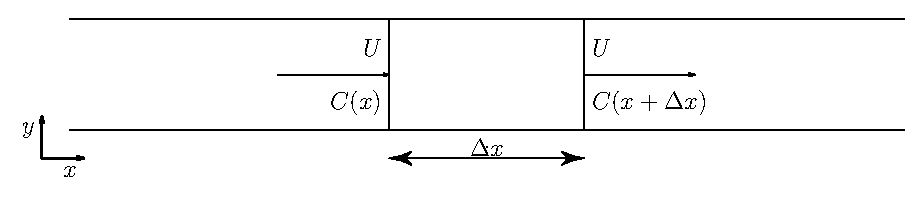
\includegraphics[width=\textwidth]{Figures/mass_transfer.eps}
\caption{The mass transfer in the moving liquid. \label{fig:moving:frame}}
\end{figure}

The mass accumulated in the unit volume $V=A \Delta x$ can be calculated as the difference of 
mass fluxes entering and leaving domain $U \bigl(C(x+\Delta x)-C(x)\bigr)$. We assume that the
source is a point source with the effective perimeter P. The accumulated mass should be proportional
to the mass transfer coefficient:
\beq
U \bigl(C(x+\Delta x)-C(x)\bigr)=k_L P \bigl(C^{*}-C(x)\bigr), 
\feq 
giving the same equation but only in the coordinate domain:
\beq
C(x)= C^{*}\Bigl(1-\exp\bigl(-k_L a \frac{x}{U} \bigr)\Bigr).
\label{main:mass:transfer:expression} 
\feq

\item If one transfers to the frame moving with the liquid velocity $U$, then the situation will be
the same as in the first case. However, one can connect the time and spatial location with the
velocity $U$ ($t=\frac{x}{U}$) to obtain the same equation as in the case 2.
\end{enumerate}

The expression (\ref{main:mass:transfer:expression}) was used in the experiments by
\citet{bercic-mass}. One should be accurate with the definition of velocities because we have two
different phases. Usually, one can take the velocity $U$ to be as
average velocity or $U=U_{gas}+U_{liq}$, where $U_{gas}$ and $U_{liq}$ are liquid and gas
superficial velocities correspondingly. In this case, the continuouty assumption is restored and
all considerations above are valid.

 However, if one wants to analytically estimate the mass transfer coefficients, the situation is
much more complicated because of the two phases presence. Phases can have different mixing patterns
from film to slug and from slug to film. The analytical approaches described above assume that the
contributions from film and bubble caps can be calculated separately. However one can see that such 
an assumption for bubble caps (slug well mixed and the concentration is uniformly distributed over
the slug) usually overpredicts the mass transfer \cite{irandoust}. This happens since some tracer
concentration from film is mixed with the slug and changes the overall concentration in the slug.
Another issue is that if the slug is long enough then the film saturates with the tracer
concentration and its influence on the mass transfer can be negligible \cite{vanbaten-circular}.
Mixing patterns of the film and the liquid slugs are of great importance for the analytical
estimation of the mass transfer \cite{yue-mass}.
 
\subsection{Numerical calculation}
In the numerical simulation it is not possible to simulate really long domains with the infinite
number of the bubbles. As we saw before there are two approaches towards it - either to simulate
the bubble train and then to measure concentration along the pipe, Eq.
\ref{main:mass:transfer:expression}, or to transfer to the reference frame moving with bulk
velocity $U$ and conduct the same measurements through Eq. \ref{main:mass:transfer:expression}.
However, both methods do require a tracking of moving bubbles which is complicated from the
numerical point of view.

Therefore, one needs to come up with the simple smaller domain calculations
of the mass transfer coefficient, which represent the continuous picture with infinite numbers of
the bubbles closely. In comparison with analytical estimations of the mass transfer coefficient,
where the mixing patterns are extremely important, the numerical simulations need only to mimic
the continous picture and provide the way to calculate the volumetric mass transfer coefficient. 

We perform simulations in the frame moving with the bubble (velocity
$U_{bubble}$), that the bubble position stands steady. The bubble velocity $U_{bubble}$ is
different from the bulk velocity $U_{gas}+U_{liq}$. In this case we need to perform coordinate
change:
\beqal
&x(t)=U_{bubble}t\\
&C(x)=C^{*}\Bigl(1-\exp\bigl(-k_L\, a \frac{x}{U_{gas}+U_{liq}}\bigr)\Bigr)\\
&C(t)=C^{*}\Bigl(1-\exp\bigl(-k_L\, a\, t \frac{U_{bubble}}{U_{gas}+U_{liq}}\bigr)\Bigr)
\feqal
If the unit volume that we simulate is quite long one can obtain the values of the concentration
in the inlet and outlet as a function of time:
\beqal
&C(U_{bubble}\, t)=C^{*}\Bigl(1-\exp\bigr(-k_L\, a\, t
\frac{U_{bubble}}{U_{gas}+U_{liq}}\bigr)\Bigr)\\
&C(U_{bubble}\,t+L_{unit})=C^{*}\Bigl(1-\exp\bigl(-k_L a \frac{
U_{bubble}\,t+L_{unit}}{U_{gas}+U_{liq}}\bigr)\Bigr)\\
&=C^{*}\Bigl(1-\exp\bigl(-k_L\, a\, t \frac{U_{bubble}}{U_{gas}+U_{liq}}\bigr)\exp\bigl(-k_L a
\frac{L_{unit}}{U_{gas}+U_{liq}}\bigr)\Bigr)
\feqal
Therefore the mass transfer coefficient can be calculated as follows:
\begin{equation}
\label{theor:continuous:mass:transfer}
\begin{aligned}
&-k_L a \frac{L_{unit}}{U_{gas}+U_{liq}}=\ln\Bigl(\frac{C^{*}-C_{outlet}}{C^{*}-C_{inlet}}\Bigr)\\
&k_L a
=\frac{U_{gas}+U_{liq}}{L_{unit}}\ln\Bigl(\frac{C^{*}-C_{inlet}}{C^{*}-C_{outlet}}
\Bigr)
\end{aligned}
\end{equation}
If inlet and outlet concentrations are small in comparison with the saturation concentration $C^{*}$
then the expression for the volumetric mass transfer coefficitent $k_L a$ can be simplified:
\beq
\vol=\frac{\Delta C}{C^{*}} \frac{U_{gas}+U_{liq}}{L_{unit}},
\feq
where $\Delta C=C_{outlet}-C_{inlet}$. If we go to the continuous formulation by changing $L_{unit}$
to be a continuous coordinate $x$, then the following can be obtained \cite{jos-mass}:
\beq
\Delta C = C^{*} \vol \frac{x}{U_{gas}+U_{liq}}
\label{small:conc:mass:estimation}
\feq

We consider the following possibilities of conducting numerical simulations:
\begin{enumerate}
 \item 
The tracer picking up procedure can be introduced
in the manner of the considerations above. We impose the concentration at the entrance to be
constant $C(0,y)=C_{inlet}$, at the outlet we impose the outflow boundary condition $\frac{\partial
C}{\partial x}(L,y)=0$. To be compliant with the considerations above one needs to impose as well
the outflow boundary conditions for the inlet as well. However, without loss of the generality one
can impose $C_{inlet}=0$, since the walls in the reference frame
moving with the bubble are moving from the inlet to the outlet. That means that no tracer
concentration leaves domain from the inlet side, which is true for the capillary numbers larger
than $0.6$.  However, this boundary condition can not be used in the case of small capillary
numbers, since there is a strong circulation in front of the bubble. One can see the sketch of the
approach in Fig. \ref{fig:benchmark:jos}. The longer the numerical domain length the better will be
results. One can estimate the volumetric mass transfer coefficient in this case through the equation
(\ref{small:conc:mass:estimation}) for small concentrations. Note a few considerations:
\begin{itemize}
\item  The considerations above were established for the homogenous velocity field. In the case of
the non-homogenous velocity field one needs to obtain a concentration from the mass flux:
\beq
C_{outlet}=\frac{\int{U(y) C(L_{unit},y) \mathrm{d}y}}{\int{U(y) \mathrm{d}y}}.
\feq
\item Note, that one cannnot use the definition of the mass transfer coefficient as far as it
varies through the bubble due to inhomogenoities of the flow. Therefore, the volumetric mass
transfer coefficient is introduced that takes into the account the bubble geometry.
\end{itemize}
\begin{figure}
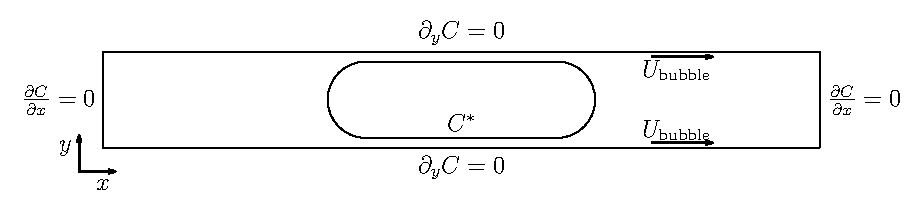
\includegraphics[width=\textwidth]{Figures/benchmark_jos.eps}
\caption{The numerical mass transfer benchmark. \label{fig:benchmark:jos}}
\end{figure}

\item Another possibility is to use the periodic boundary conditions as the limiting case of the
continuous formulation. In this case the inlet and outlet concentrations are not much different
($C(x)=C(x+L_{unit})=C(x+\Delta x)\approx C_{media}$, see Fig. \ref{fig:moving:frame}), where
$C_{media}$ is the mass averaged over domain concentration. This formulation requires the periodic
boundary condition $C_{inlet}=C_{outlet}$. By the definition the mass transfer coefficient is
proportional to the gain of the mass in the system divided by the concentration difference:
\beq
j=\frac{\dot{m}}{P \Delta C}=\frac{\dot{m}}{P (C^{*}-C_{media})},
\feq
where mass difference in the domain can be calculated as:
\beq
\dot{m}=\frac{m_2-m_1}{t_2-t_1}=\frac{\int_{C(t_2)\mathrm{d}V}-\int{C(t_1)\mathrm{d}V}}{t_2-t_1}.
\feq
Therefore the assumptions  of this approach is that the difference between inlet and outlet is not
considerably large and the tracer is well mixed in the slug, as one can take the concentration
difference as $\Delta C = C^{*}-C_{media}$. The best case scenario is when $C_{media}$ is close to
zero, in this case we can be sure that the flux to the domain is calculated precisely and periodic
boundary conditions are fulfilled.
\end{enumerate}

\section{Mass transfer}
The mass transfer is characterized by non-dimensional numbers as Schmidt number (viscous diffusion
rate over mass diffusion rate), the Peclet number (convection over diffusion) and the Sherwood
number (convection mass transfer over diffusion mass transfer):
\begin{equation}
\begin{aligned}
&Pe=\frac{U L}{D}\\
&Sh=\frac{K L}{D}\\
&Sc=\frac{\nu}{D}\\
\end{aligned}
\end{equation}

As far as the lattice Boltzmann method operates only in the non-dimensional space, one needs to
match the non-dimensional lattice Boltzmann parameters with non-dimensional physical parameters.
Therefore, one needs to form non-dimensional numbers from the physical parameters. One of the
particular experiment examples is the
work by \citet{bercic-mass} who used the methane dissolution to characterize the mass transfer for
bubble train flow. 

In what follows we will perform the matching of obtained hydrodynamics results
\cite{kuzmin-binary2d} with physical ones from experiment of \citet{bercic-mass}. The diffusion
coefficient of the methane under standard conditions \cite{methane-properties} is
$1.84\times 10^{-5} \mathrm{cm}^2/\mathrm{s}$. The diameters of capillaries in the experiment were
as $1.5$, $2.5$ and
$3.1\,\mathrm{mm}$. For simplicity reasons we will choose the diameter of capillary as $1.5\,
\mathrm{mm}$. 
The non-dimensional parameters obtained from the hydrodynamics lattice Boltzmann simulations are
as:
\begin{equation}
\begin{aligned}
&Ca=\frac{U \mu_{\mathrm{liq}}}{\gamma}\\
&Re=\frac{\rho_{\mathrm{liq}} U L}{\mu_{\mathrm{liq}}}.
\end{aligned}
\end{equation}
Given some physical characteristics as the liquid density and the channel length,
one can obtain the physical velocity obtained from non-dimensional numbers:
\begin{equation}
\begin{aligned}
Ca\cdot Re= \frac{\rho_{\mathrm{liq}} U^2 L}{\gamma}\\
U=\sqrt{\frac{Ca\,Re\,\gamma}{\rho_{\mathrm{liq}}L}}
\end{aligned}
\end{equation}

Assuming that the surface tension of water is $0.0728\,\mathrm{N/m}$ (methane exhibits the same
trend \cite{schmidt-methane}), the density is       
$1000\,\mathrm{kg/m^3}$, the hydraulic diameter of the channel to be $1.5\,\mathrm{mm}$ one can
calculate the physical velocity of the bubble.
Table \ref{table:twod:simulations} represents lattice Boltzmann simulations results and their
physical equivalents for the grid $202\times 3002$. One can see
that velocity is quite reasonable
as \citet{bercic-mass} declared that experiments were conducted for velocities in the ranges of
$0.01$ to $0.4\,\mathrm{m}/\mathrm{s}$. 
\begin{table}
\begin{tabularx}{\textwidth}{|X|X|X|X|X|X|}
\hline
$Ca$    &$Re$     &$U_{LB}$ &$\delta$&$\varepsilon_{\mathrm{gas}}$
&$U_{\mathrm{phys}}, \mathrm{m/s}$\\
\hline
$0.026$ &$0.449$  &$0.0014$ &$0.040$ &$0.306$ &$0.023$   \\ 
$0.047$ &$0.820$  &$0.0027$ &$0.058$ &$0.293$ &$0.043$   \\ 
$0.080$ &$1.378$  &$0.0045$ &$0.085$ &$0.280$ &$0.073$ \\
$0.065$ &$1.126$  &$0.0037$ &$0.076$ &$0.266$ &$0.059$      \\
$0.222$ &$3.807$  &$0.0125$ &$0.122$ &$0.253$ &$0.202$  \\
$0.479$ &$8.222$  &$0.0271$ &$0.151$ &$0.249$ &$0.437$  \\
$0.736$ &$12.617$ &$0.0416$ &$0.164$ &$0.236$ &$0.671$  \\ 
$0.989$ &$16.960$ &$0.0559$ &$0.172$ &$0.230$ &$0.902$  \\
\hline
\end{tabularx}
\caption{Two-dimensional simulations for different
capillary numbers. \label{table:twod:simulations}}
\end{table}

\section{Lattice Boltzmann implementation}
For the lattice Boltzmann implementation we took $\omega=1.99$ which results in the following
lattice Boltzmann diffusivity parameter:
\begin{equation}
\begin{aligned}
&D=\frac{1}{3}\Bigl(\frac{1}{\omega}-\frac{1}{2}\Bigr)\\
&D=0.0008375
\end{aligned}
\end{equation}
In terms of the Schmidt number (taking the lattice Boltzmann liquid viscosity in former simulations
as $\frac{2}{3}$) that
can result in:
\begin{equation}
\begin{aligned}
&Sc=\frac{\nu_{\mathrm{liq}}}{D}\\
&Sc=796\\
\end{aligned}
\end{equation}
Taking the water dynamic viscosity as $8.9 \times 10^{-4}\,\mathrm{Pa\cdot s}$ or kinematic
viscosity as $8.9 \times
10^{-7} \,\mathrm{m^2/s}$ and the Schmidt number as $796$ results in the following physical
diffusion coefficient:
\begin{equation}
D=1.118\times 10^{-5}\,\mathrm{cm^2/s},
\end{equation}
which is less than the diffusivity of the methane $1.84\times 10^{-5}\,\mathrm{cm^2/s}$ but is
physical. After calculation of physical parameters one can calculate correlations indicated in
Section \ref{sec:correlations} for mass transfer. Table \ref{table:lengths} presents extraction
from the lattice Boltzmann simulation necessary to calculate mass transfer calculations.
For the two-dimensional case parameter  $a$ is defined as:
\begin{equation}
a = \frac{\text{bubble perimeter}}{\text{cell area}}.
\end{equation}
For the height of the channel to be $H=1.5 \times 10^{-3}\,\mathrm{m}$, parameters $a$ are
presented in Table \ref{table:lengths}. 
\begin{table}
\begin{tabularx}{\textwidth}{|X|X|X|X|X|X|}
\hline
$Ca$&Bubble length& Slug Length&
$U_{\mathrm{gas}},\,\mathrm{m/s}$&$U_{\mathrm{liq}},\,\mathrm{m/s}$&$a,\,\mathrm{m^{-1}}$\\
\hline
$0.026$&$5.225$&$9.775$ &$0.0070$ &$0.0209$&$510.77$\\
$0.047$&$5.22$ &$9.78$  &$0.0126$ &$0.0379$&$508.62$\\
$0.080$&$5.215$&$9.785$ &$0.0204$ &$0.0615$&$506.53$\\
$0.065$&$4.965$&$10.035$&$0.0157$ &$0.0504$&$482.84$\\
$0.222$&$5.25$ &$9.75$  &$0.0511$ &$0.1560$&$505.06$\\
$0.479$&$5.565$&$9.435$ &$0.1089$ &$0.3155$&$530.37$\\
$0.736$&$5.51$ &$9.49$  &$0.1584$ &$0.4677$&$525.38$\\
$0.989$&$5.505$&$9.495$ &$0.2074$ &$0.6190$&$526.80$\\
\hline
\end{tabularx}
\caption{The nondimensional (scaled to the height of the channel) lengths for the same
lattice Boltzmann simulations as in Table \ref{table:twod:simulations}. As well superficial
gas and liquid velocities are presented. \label{table:lengths}} 
\end{table}

The literature correlations of mass transfer dependence on the bubble velocities are presented in
Fig. \ref{fig:mass:transfer:theoretical}. Note, that the correlations presented in
Fig. \ref{fig:mass:transfer:theoretical} are used primarily for circular capillaries
(\citeauthor{vanbaten-circular,bercic-mass}) and for square capillaries (\citeauthor{yue-mass}). We
adapt these results for flow between parallel plates by using hydraulic
diameter \cite{bercic-mass} which can be calculated as:
\begin{equation}
d_h = \lim_{W\to\infty}\frac{4A}{P}=\lim_{W\to\infty}\frac{4 W\,H}{2(W+H)}=2 H.
\end{equation}
For comparison reasons we derived in Section \ref{mass:transfer:correlation} the correlation for the
flow between plates, see Fig. \ref{fig:mass:transfer:theoretical}. One can see that the
difference is negligible.

\begin{figure}[htb!]
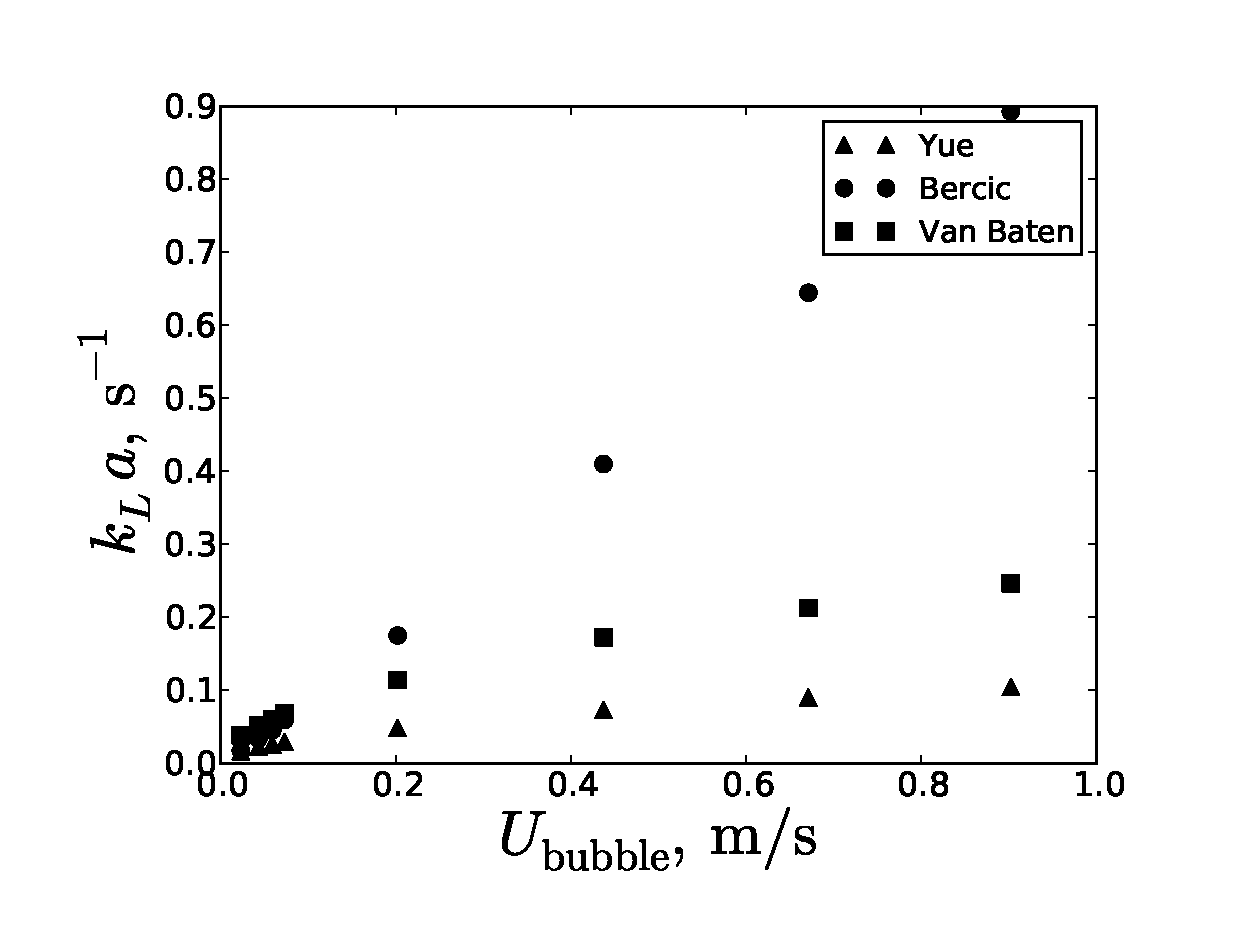
\includegraphics[width=\textwidth]{Figures/theoretical_correlations.eps}\\
%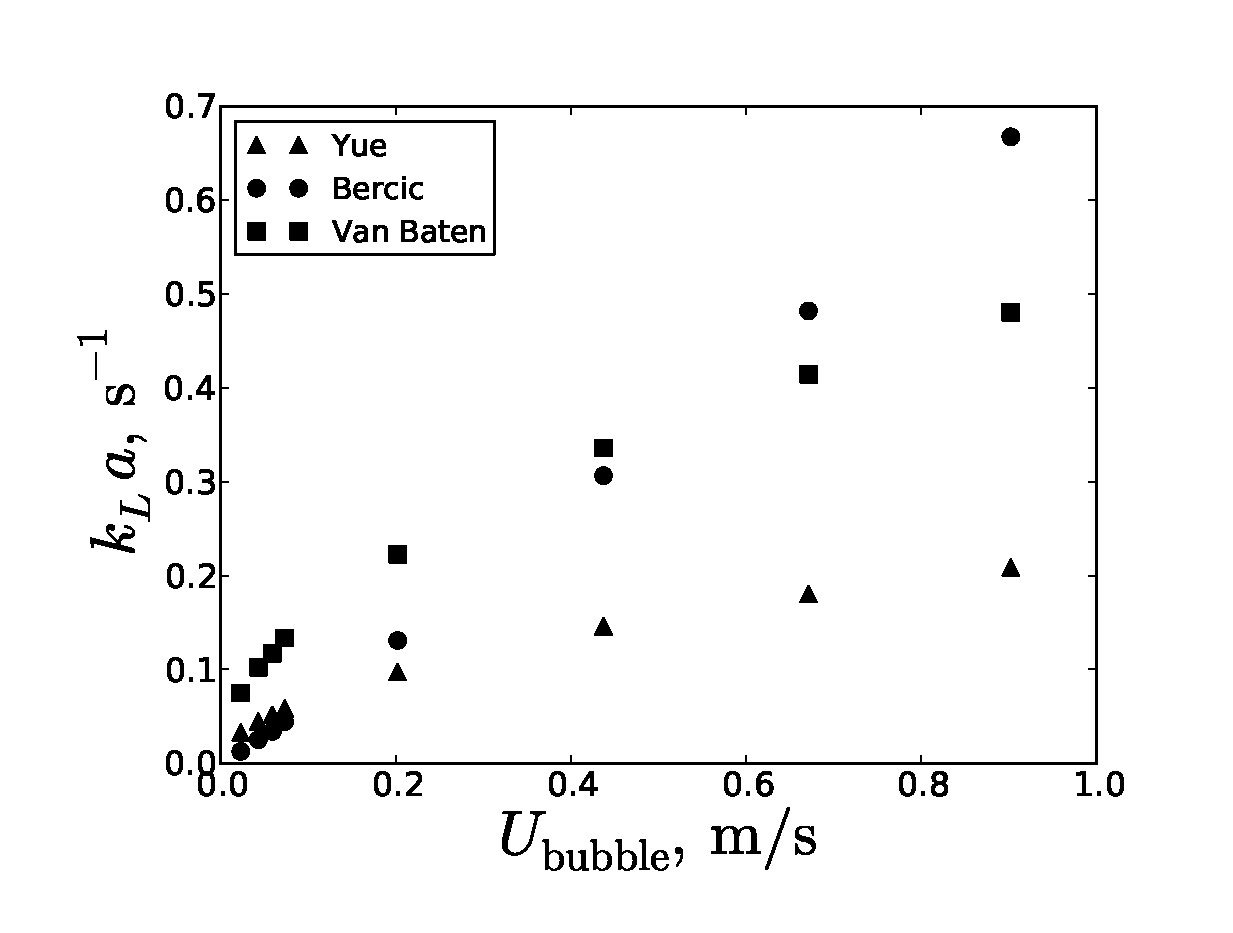
\includegraphics[width=\textwidth]{Figures/theoretical_correlations_without_hydraulic.eps}\\
\caption{The literature correlations by various authors.\label{fig:mass:transfer:theoretical}}
\end{figure}

The volumetric mass transfer coefficient is calculated according to the work of
\citet{vanbaten-circular}. The concentration flux is calculated as the difference between overall
average concentration taken in the whole domain ($C_{overall}=\int_{V} C \mathrm{d}V /V$)
at time
$t_1$ and time $t_2$ divided on the time difference $t_2-t_1$ {\color{red} (In this particular
moment I don't know whether to take the volume of the whole domain or
just the liquid phase. I will go for whole domain.)}. Then the volumetric mass transfer
coefficient is calculated as \cite{vanbaten-circular}:
\begin{equation}
\label{main:simulation:equation}
k_L a=\frac{\text{Flux}}{C_s-C_{outlet}} \frac{\text{bubble surface area}}{\text{unit cell volume}},
\end{equation}
where $C_{outlet}=\int{C U_{outlet}\mathrm{d}A}/\int{U_{outlet}\mathrm{d}A}$. 
{\color{red} Do not understand why we need this ratio bubble surface area/unit cell volume. In this
case the dimensional units do not coincide. In the calculations I will avoid it until further
clearance.} The overall concentration in the lattice Boltzmann system is prescribed as:
\begin{equation}
C_{overall}=\frac{\sum{c_i}}{N_x \, (N_y-2)}.
\end{equation}

To properly do
non-dimensioanalization one needs to insure the time conversion factor when the flux is calculated
inside the lattice Botlzmann system. The time conversion can be easily obtained:
\begin{equation}
\begin{aligned}
&U_{LB}=U_{phys}\frac{\Delta t}{\Delta x}\\
&\Delta t=\frac{U_{LB}}{U_{phys}}\Delta x\\
&\Delta t=\frac{1.5\,\mathrm{mm}}{200} \frac{0.0559}{0.902\,\mathrm{m/s}}=4.64\times
10^{-7}\,\mathrm{s} 
\end{aligned}
\end{equation}

The bubble surface length is the perimeter of the bubble in two-dimensional space and it is
calculated with the extraction of the bubble contour and representing it with the polygon. After
that the calculated perimeter is the effective summation of line lengths and can be represented as:
\begin{equation}
P=\sum_i{\sqrt{(x2_i-x1_i)^2+(y2_i-y1_i)^2}},
\end{equation}
where the index $i$ represents the polyline consisting of two points $(x1,y1)$ and $(x2,y2)$.
%The corresponding volumetric mass transfer coefficients depending on the velocity are indicated in
%Table \ref{table:volumetric:coefficients}.

\section{Comparison between different approaches for one unit cell}
We consequently will examine different approaches to the mass transfer definition, Fig.
\ref{fig:comparison:one:unit:cell}:
\begin{description}
\item[I] Definition of \citet{vanbaten-circular} with periodic boundary conditions where a bubble
is located near the entrance of the computational domain, and the characteristic concentration is
the inlet/outlet concentration, Fig \ref{fig:benchmark}. 
\item[II] Definition of \citet{vanbaten-circular} with periodic boundary conditions where a bubble
is located near the entrance of the computational domain, and the characteristic concentration is
the average concentration, Fig \ref{fig:benchmark}.
\item[III] Definition of \citet{vanbaten-circular} with periodic boundary conditions where a
bubble is located in the middle of the computational domain, and the characteristic concentration
is the inlet/outlet concentration.
\item[IV] Definition of \citet{vanbaten-circular} with periodic boundary conditions where a bubble
is located in the middle of the computational domain, and the characteristic concentration is the
average concentration.
\item[V] Definition with the concentration jump between inlet and outlet over one unit cell.
\end{description}
\begin{figure}[htb!]
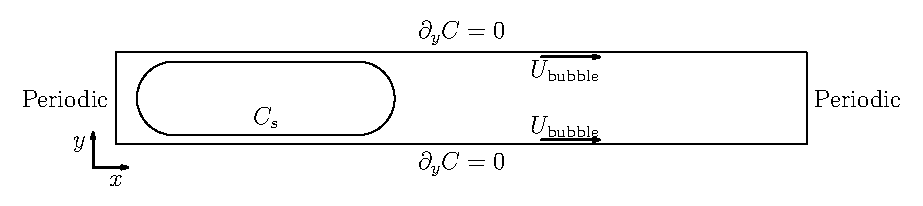
\includegraphics[width=\textwidth]{Figures/benchmark_periodic.eps}\\
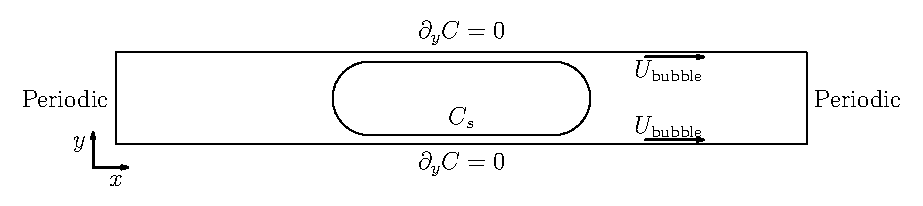
\includegraphics[width=\textwidth]{Figures/benchmark_middle.eps}\\
\caption{The two-dimensional benchmarks for the  the mass transfer
coefficient (bottom) for the bubble located near the entrance (top) and at the middle of the domain
(bottom). \label{fig:benchmark}}
\end{figure}

\begin{figure}[htb!]
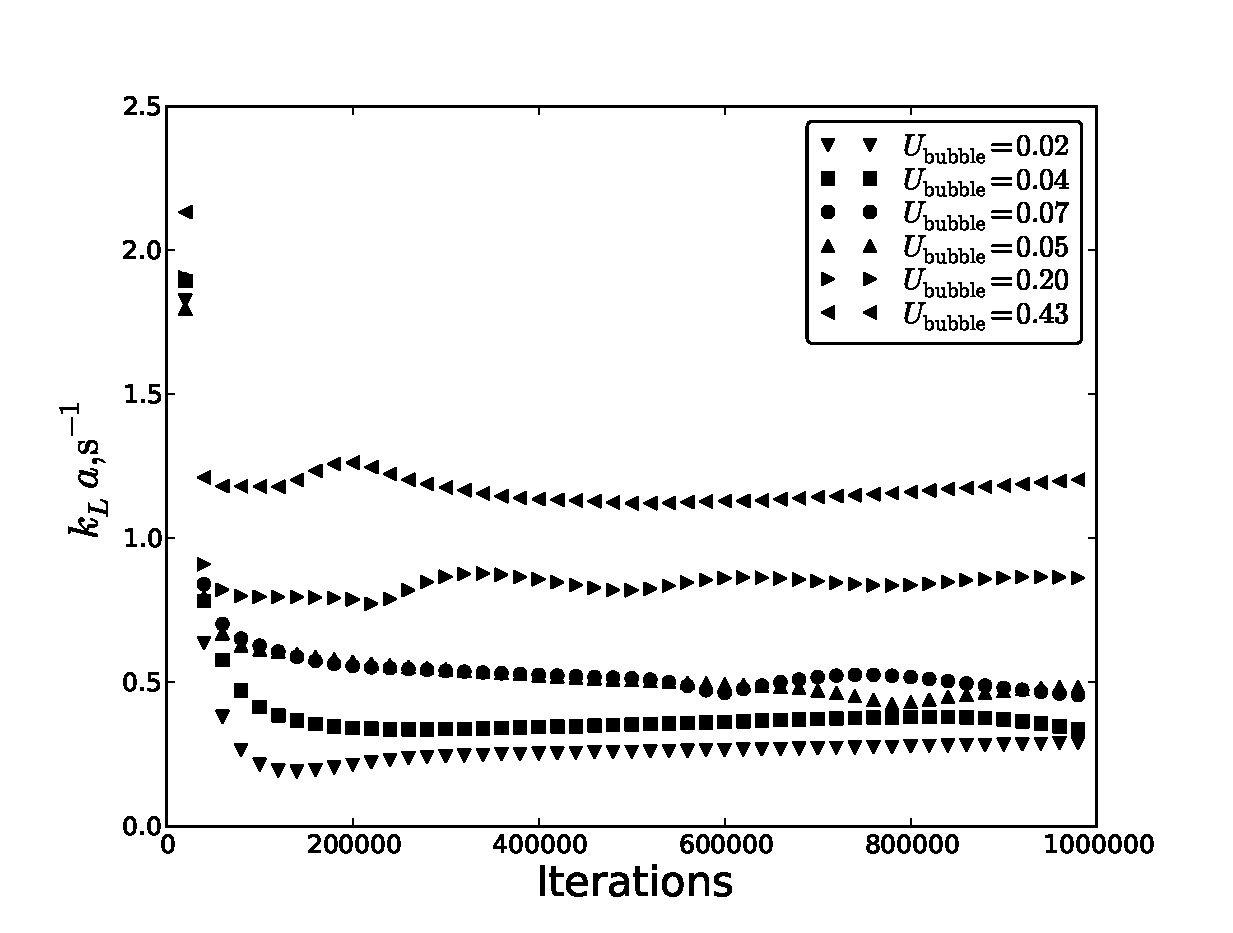
\includegraphics[width=0.5\textwidth]{Figures/steady_state_per_entrance.eps}
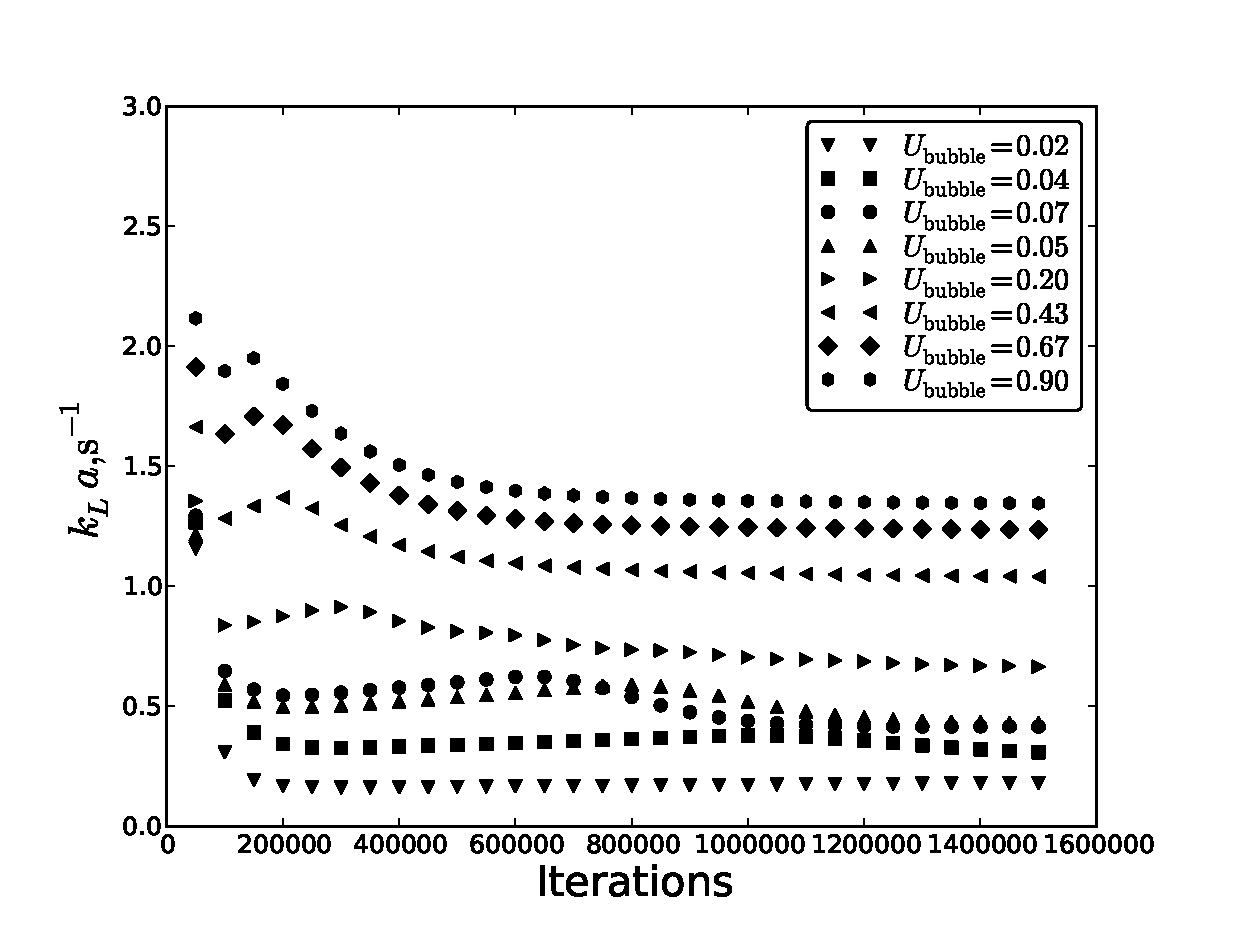
\includegraphics[width=0.5\textwidth]{Figures/steady_state_inlet_aver.eps}\\
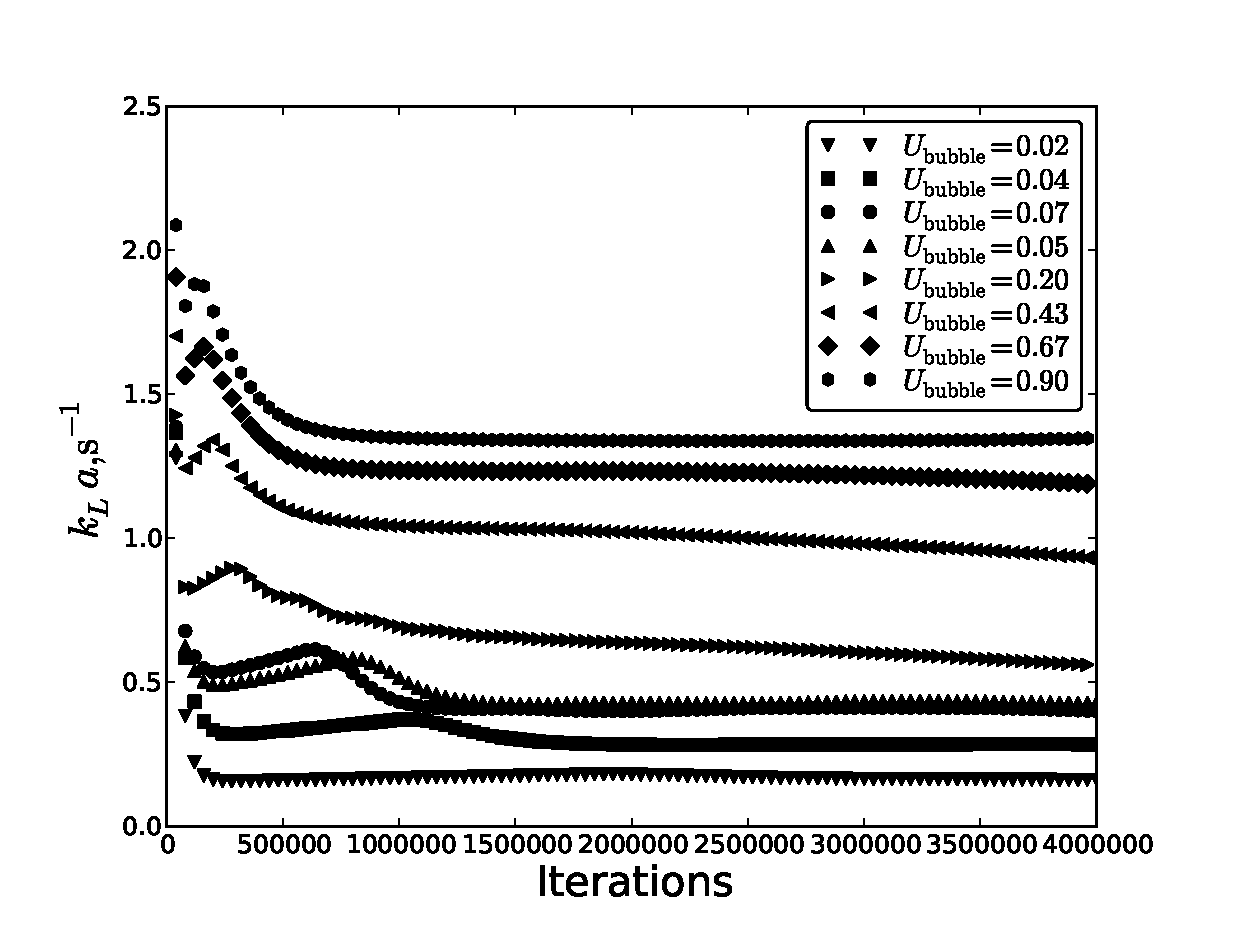
\includegraphics[width=0.5\textwidth]{Figures/steady_state_per_aver.eps}
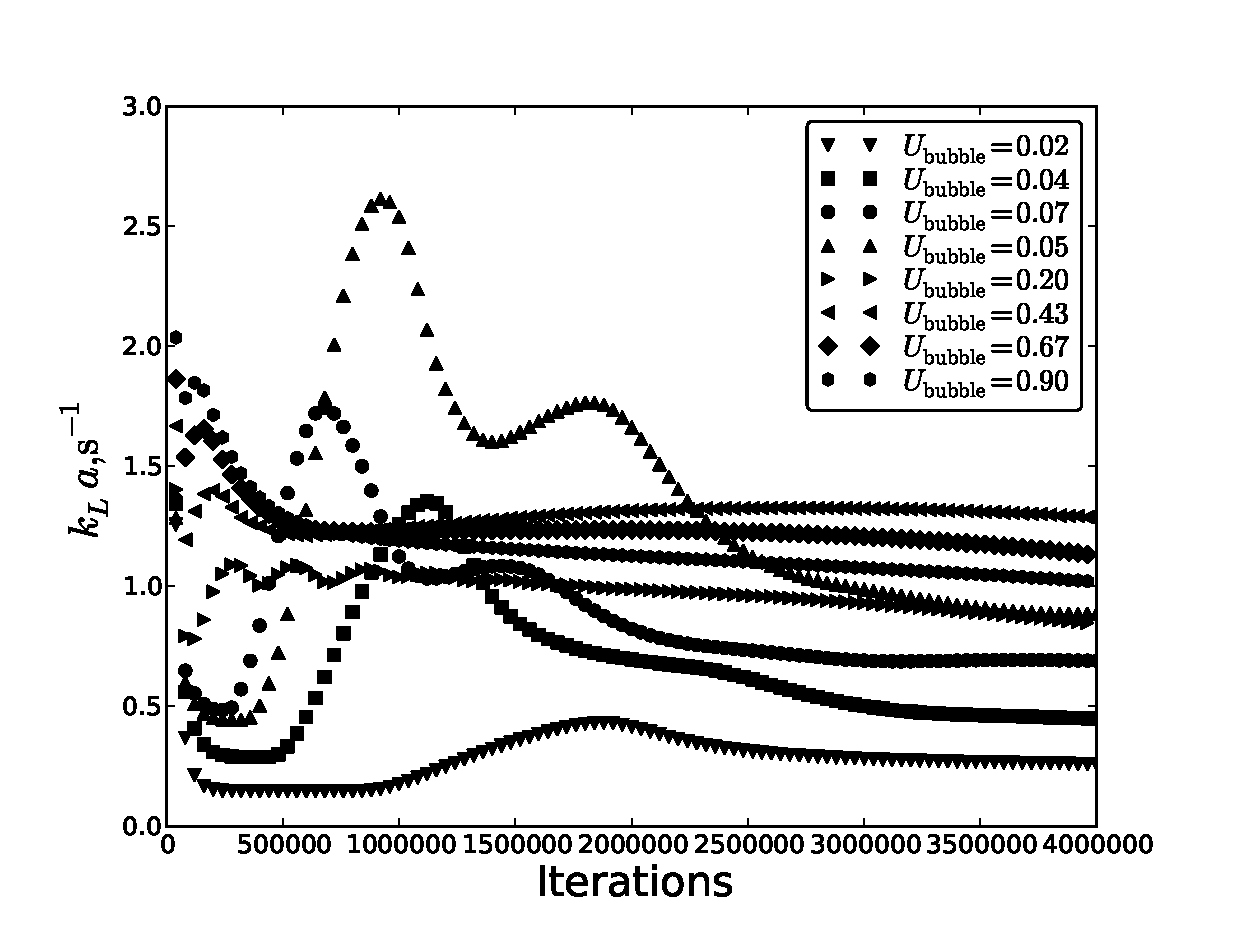
\includegraphics[width=0.5\textwidth]{Figures/steady_state_per_middle_outlet.eps}\\
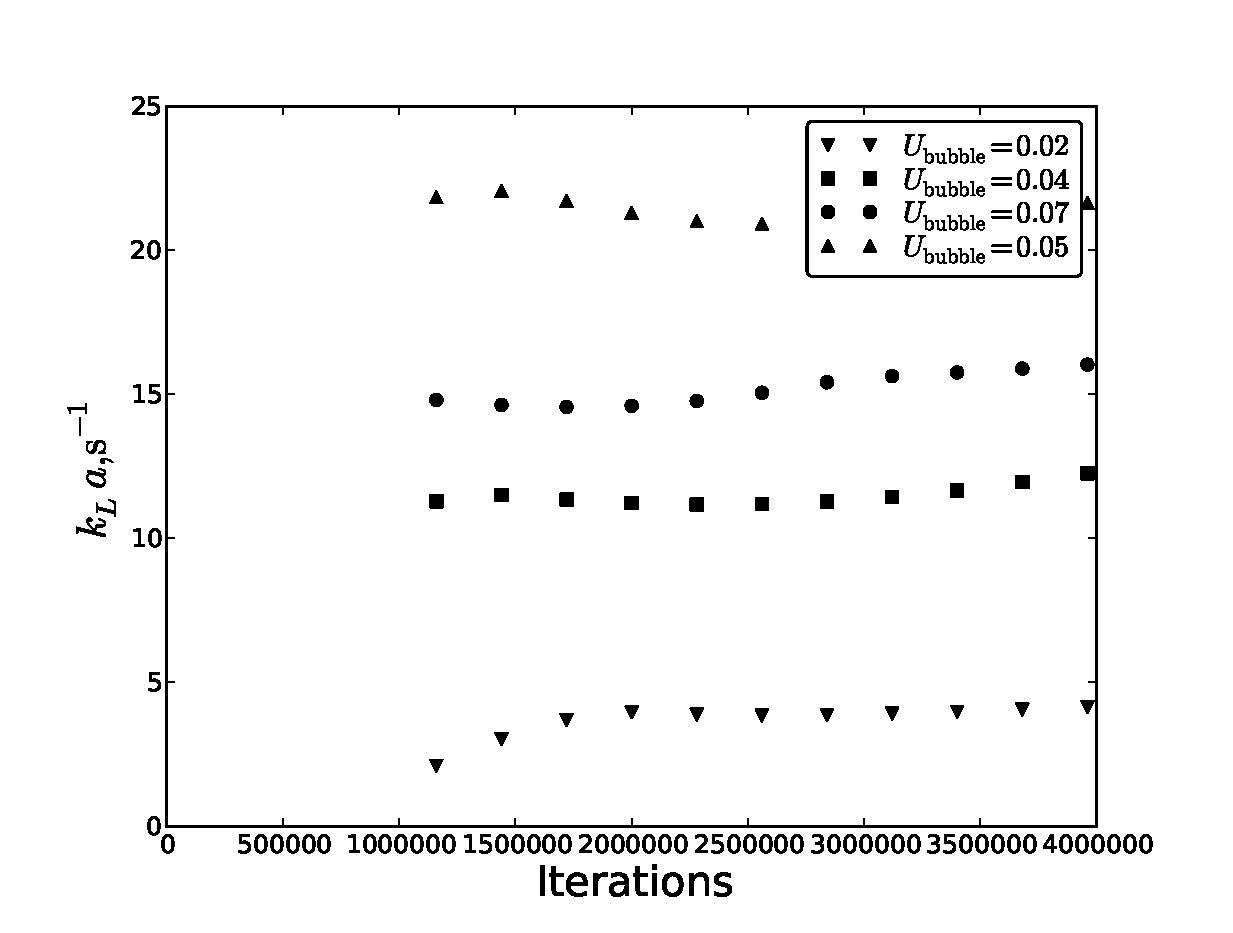
\includegraphics[width=0.5\textwidth]{Figures/steady_state_jos_inlet_outlet.eps}\\
\caption{\label{fig:comparison:one:unit:cell}}
\end{figure}
All the comparison is summarized in Table \ref{table:one_unit_comparison}.
\begin{table}[htb!]
\begin{tabularx}{\textwidth}{|X|X|X|X|X|X|X|X|}
\hline
$Ca$&$Fo$&$\vol_{ent},\,\mathrm{s}^{-1}$&$\vol_{aver},\,\mathrm{s}^{-1}$&$\vol_{mid,
aver},\,\mathrm{s} ^ { -1 }$&$\vol_{mid,out},\,\mathrm{s}^{-1}$&$\vol_{open},\,\mathrm{s}^{-1}$ \\
\hline
$0.026$&$0.08493$&$0.2737$&$0.1775$&$0.1692$&$0.2631$&$3.6756$\\
$0.047$&$0.02160$&$0.3664$&$0.3431$&$0.2852$&$0.4553$&$11.4822$\\
$0.080$&$0.00588$&$0.4959$&$0.4185$&$0.4079$&$0.6920$&$15.1964$\\
$0.065$&$0.00862$&$0.4734$&$0.4517$&$0.4303$&$0.8923$&$21.4517$\\
$0.222$&$0.00103$&$0.8505$&$0.6799$&$0.6109$&$0.8679$&N/A\\
$0.479$&$0.00034$&$1.1541$&$1.0460$&$0.9884$&$1.2995$&N/A\\
$0.736$&$0.00018$&$1.1801$&$1.2395$&$1.2199$&$1.1555$&N/A\\
$0.989$&$0.00012$&$1.2215$&$1.3493$&$1.3400$&$1.0350$&N/A\\
\hline
\end{tabularx}
\caption{Simulation results for different capillary numbers.
\label{table:one_unit_comparison}}
\end{table}
One can see that the only consistent result is for simulations which take into the account average
concentration. The results come to the steady-state after $1,000,000$ iterations. However, to
understand properly what is the real mass transfer coefficient one needs to perform a few units
simultions.

\section{Two unit cells results}
As far as one needs to restore the continuous picture one needs to make a simulation of a few
cells. This section provides results for two units. The results are summarized in Table
\ref{table:two_units}. The results for two sections are presented in Fig. \ref{fig:results:double}.
\begin{figure}[htb!]
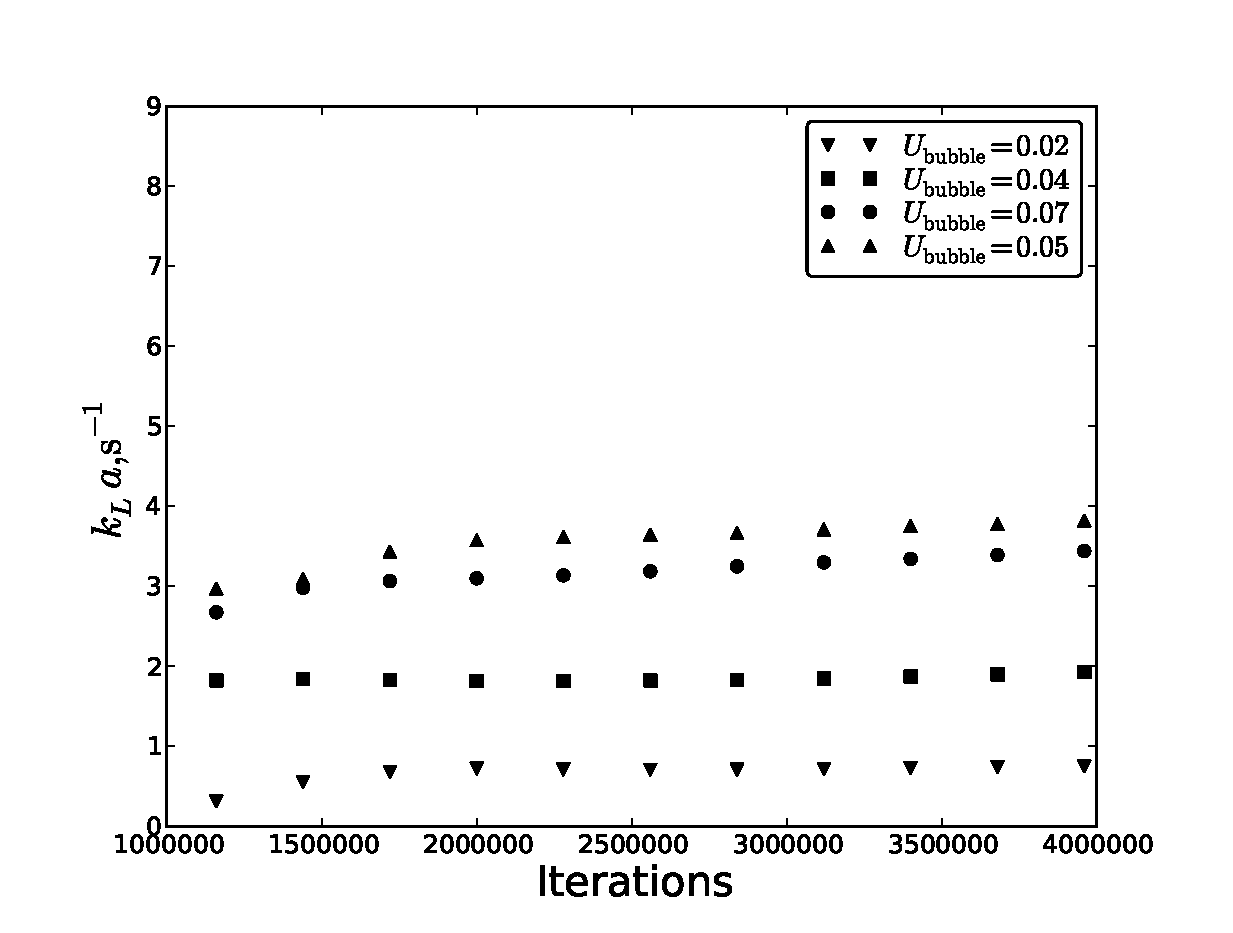
\includegraphics[width=0.5\textwidth]{Figures/steady_double_overall.eps}
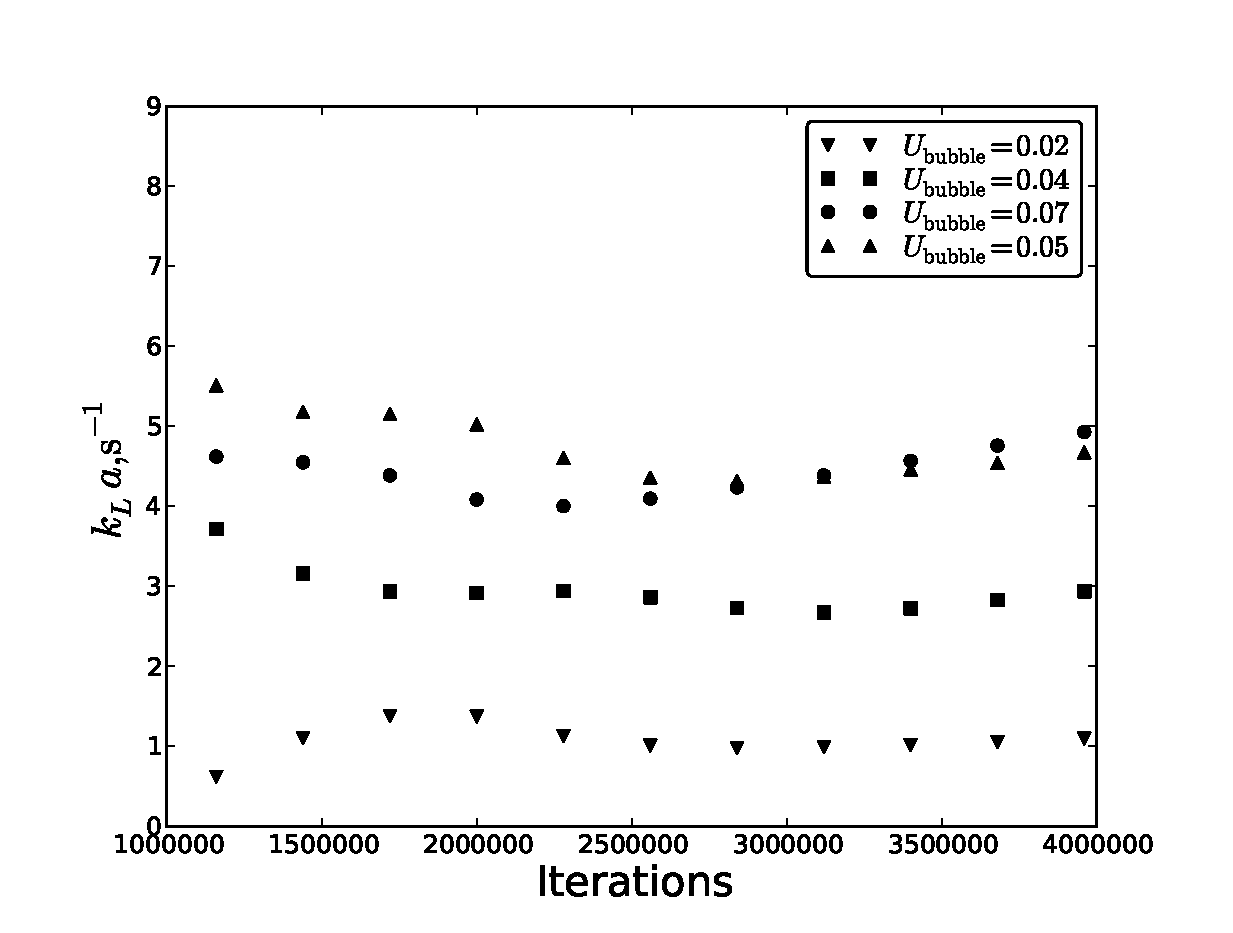
\includegraphics[width=0.5\textwidth]{Figures/steady_double_first.eps}\\
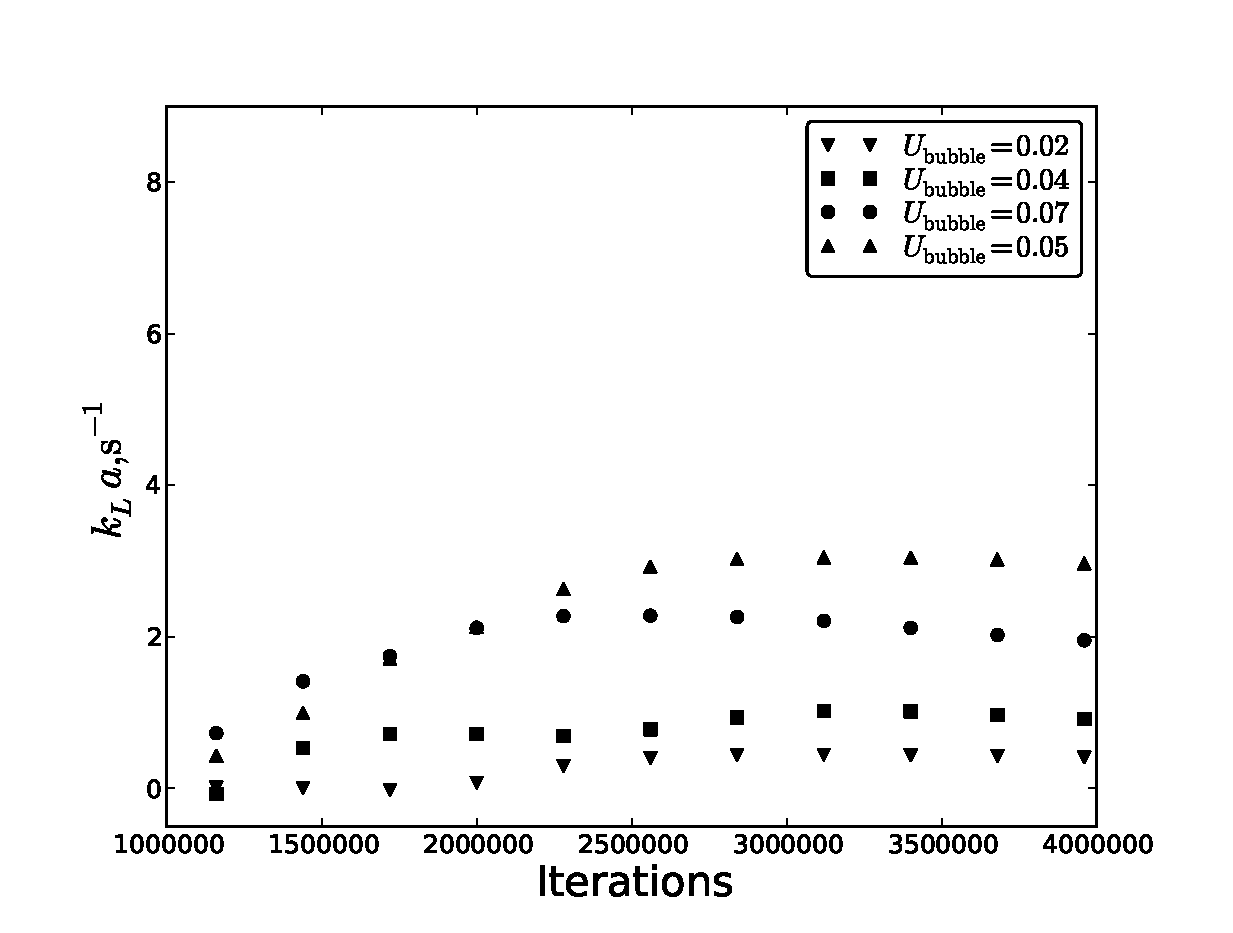
\includegraphics[width=0.5\textwidth]{Figures/steady_double_second.eps}
\caption{Overall mass transfer coefficient (top left), first part (top
right), second part (bottom left).\label{fig:results:double}}
\end{figure}
\begin{table}[htb!]
\begin{tabularx}{\textwidth}{|X|X|X|}
\hline
$0.7392$&$1.0564$&$0.4220$\\
$1.8993$&$2.8301$&$0.9684$\\
$3.3925$&$4.7522$&$2.0328$\\
$3.7870$&$4.5615$&$3.0125$\\
\hline
\end{tabularx}
\caption{Simulation results for two units. \label{table:two_units}}
\end{table}

\section{Three unit cells results}
Three unit cells results are subdivided into three cells. We calculate the mass transfer
coefficients over the each cell, Fig. \ref{fig:results:triple}. The averaged coefficients  after
$3,300,000$ time steps are represented in Table. \ref{table:three_units}. The most important thing
is to look at the third column of the Table \ref{table:three_units} or for at the Fig.
\ref{fig:results:triple} (bottom left). The coefficients for capillary numbers $0.026$ and $0.047$
are almost zero which indicates that the concentration at the first part of the channel is almost
the same as the second part. Thus, there is not enough time steps to transfer concentrate among
whole the channel (plug flow). In comparison with the first two values for capillary number $0.080$
the trend is different and concentrate is spread over the channel. However, the drop coefficients
are still inconsistents. Though last part and the second part exhibit close values (needed to tell
what is the real mass transfer coefficient). Overall, more time steps are needed.
$0.080$
\begin{table}[htb!]
\begin{tabularx}{\textwidth}{|X|X|X|X|}
\hline
0.4928&1.0564&2.8472e-05&0.4219\\
1.2662&2.8301&0.0146&0.9537\\
2.3110&4.7532&1.0665&1.1133\\
\hline
\end{tabularx}
\caption{Simulation results for three units.\label{table:three_units}}
\end{table}
\begin{figure}[htb!]
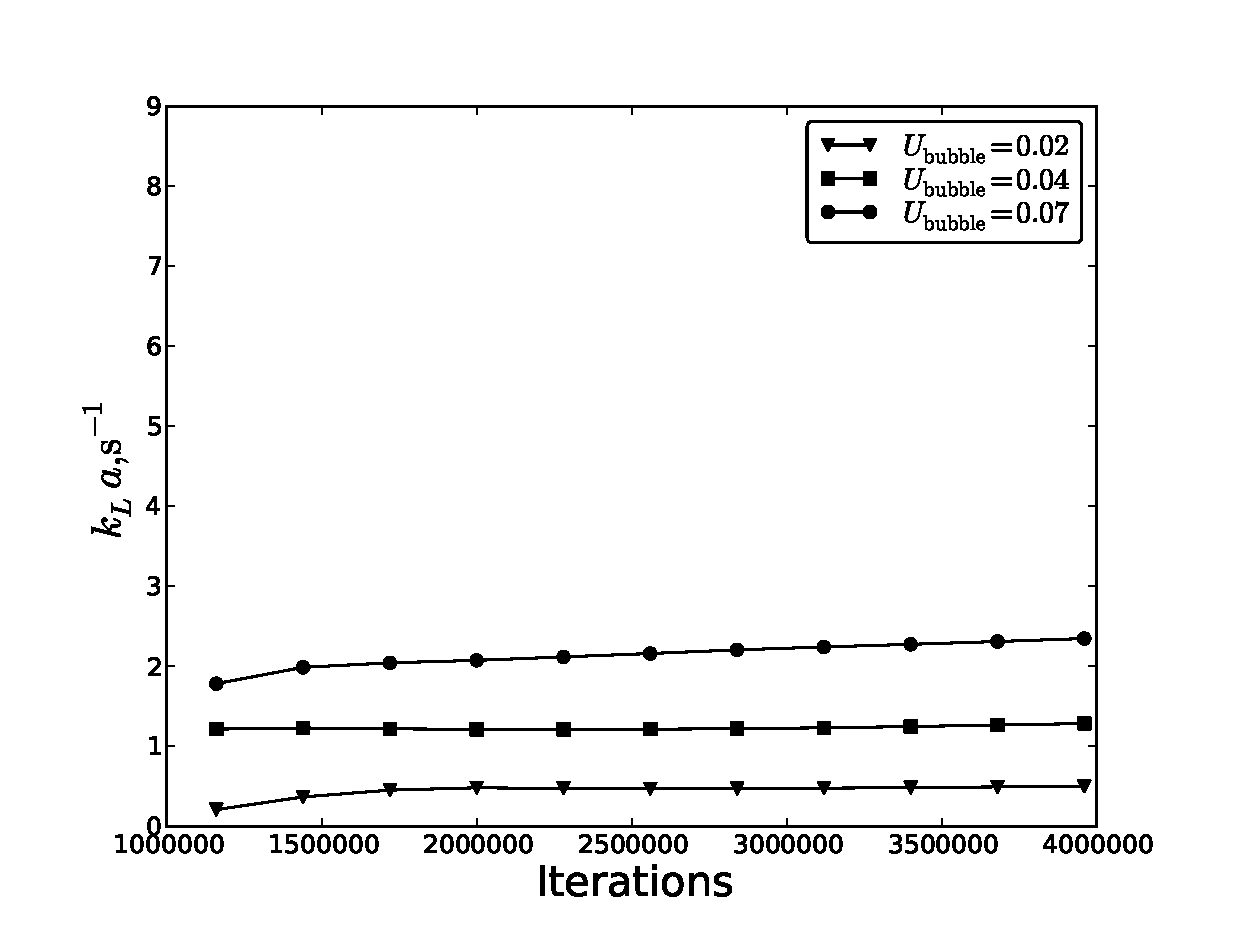
\includegraphics[width=0.5\textwidth]{Figures/steady_triple_overall.eps}
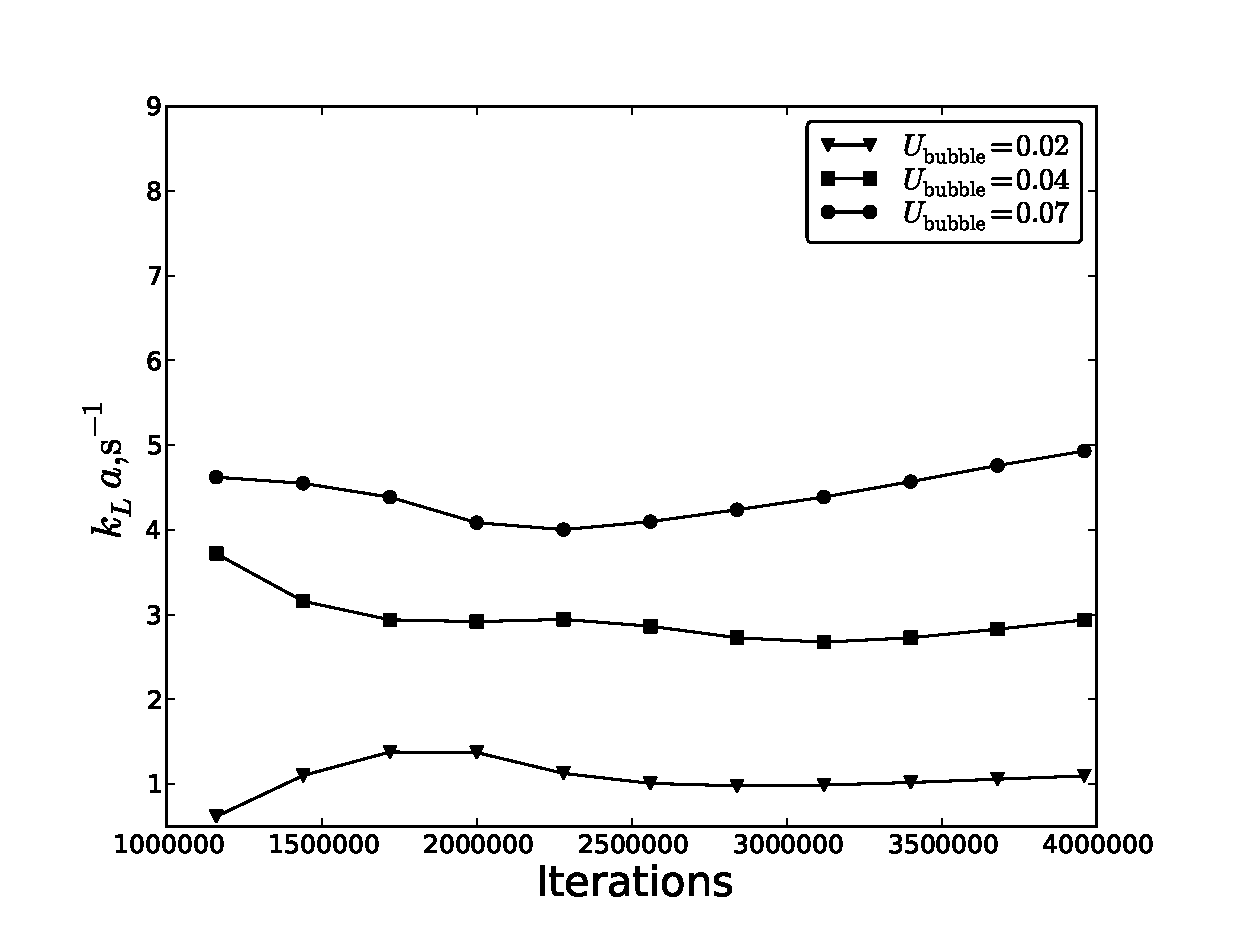
\includegraphics[width=0.5\textwidth]{Figures/steady_triple_first.eps}\\
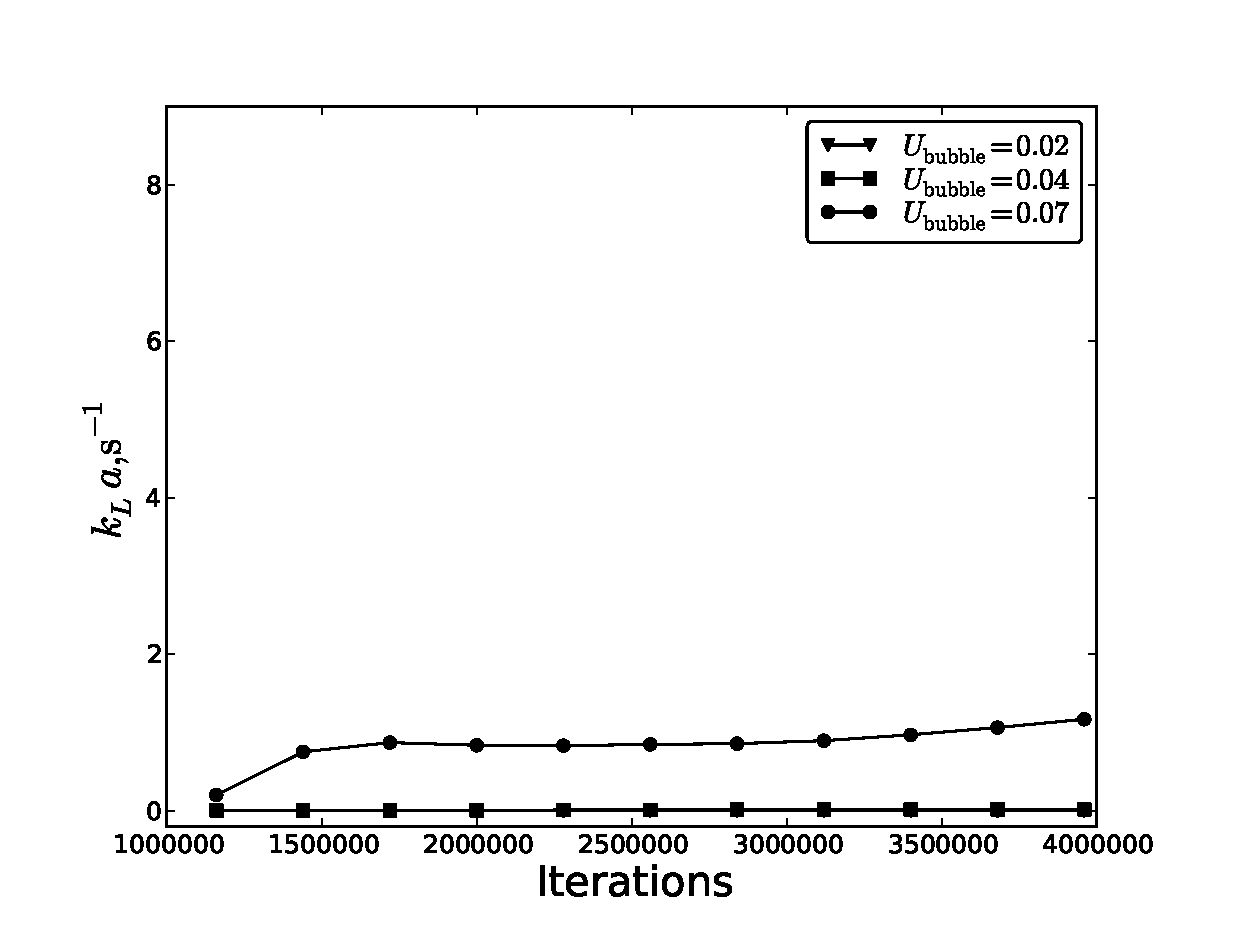
\includegraphics[width=0.5\textwidth]{Figures/steady_triple_second.eps}
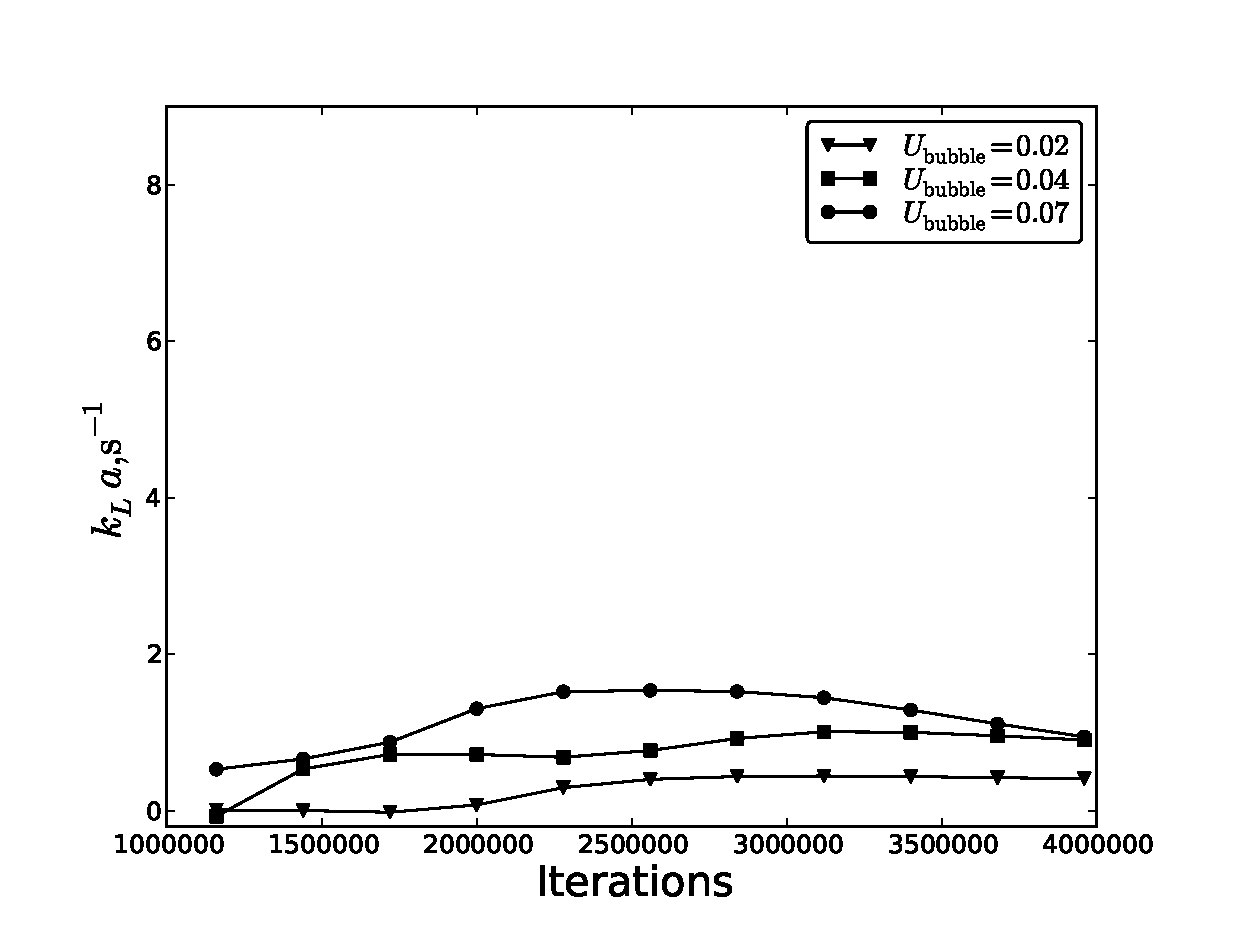
\includegraphics[width=0.5\textwidth]{Figures/steady_triple_third.eps}\\
\caption{The mass transfer coefficient over time in different locations: overall mass transfer
coefficient (top left), first part (top right), second part (bottom left), third part (bottom
right). \label{fig:results:triple}}
\end{figure}

{\color{red} Probably we can consider that for capillary number less than $0.08$ the mass transfer
is a plug flow mass transfer, keeping only the impact from caps.}

\section{Four unit cells results}
Four unit cells results are subdivided into four cells. The results are presented in Fig.
\ref{fig:results:quadro}. While we expect certain deviations for the first and the last part, but
surprisingly the concentration difference over the third segment tends to be zero. That means not
enough time steps are performed. The results over segments are summarized in Table
\ref{table:four_units}.
\begin{table}[htb!]
\begin{tabularx}{\textwidth}{|X|X|X|X|X|X|}
\hline
$Ca$   &Overall  &I       &II      &III     &IV\\
$0.080$&$1.7359$ &$4.7533$&$1.0665$&$0.1088$&$1.0150$\\
$0.065$&$1.9260$ &$4.5620$&$0.9113$&$0.0619$&$2.1689$\\
\hline
\end{tabularx}
\caption{Simulation results for mass transfer coefficients for 4 unit cells
domain.\label{table:four_units}}
\end{table}
\begin{figure}[htb!]
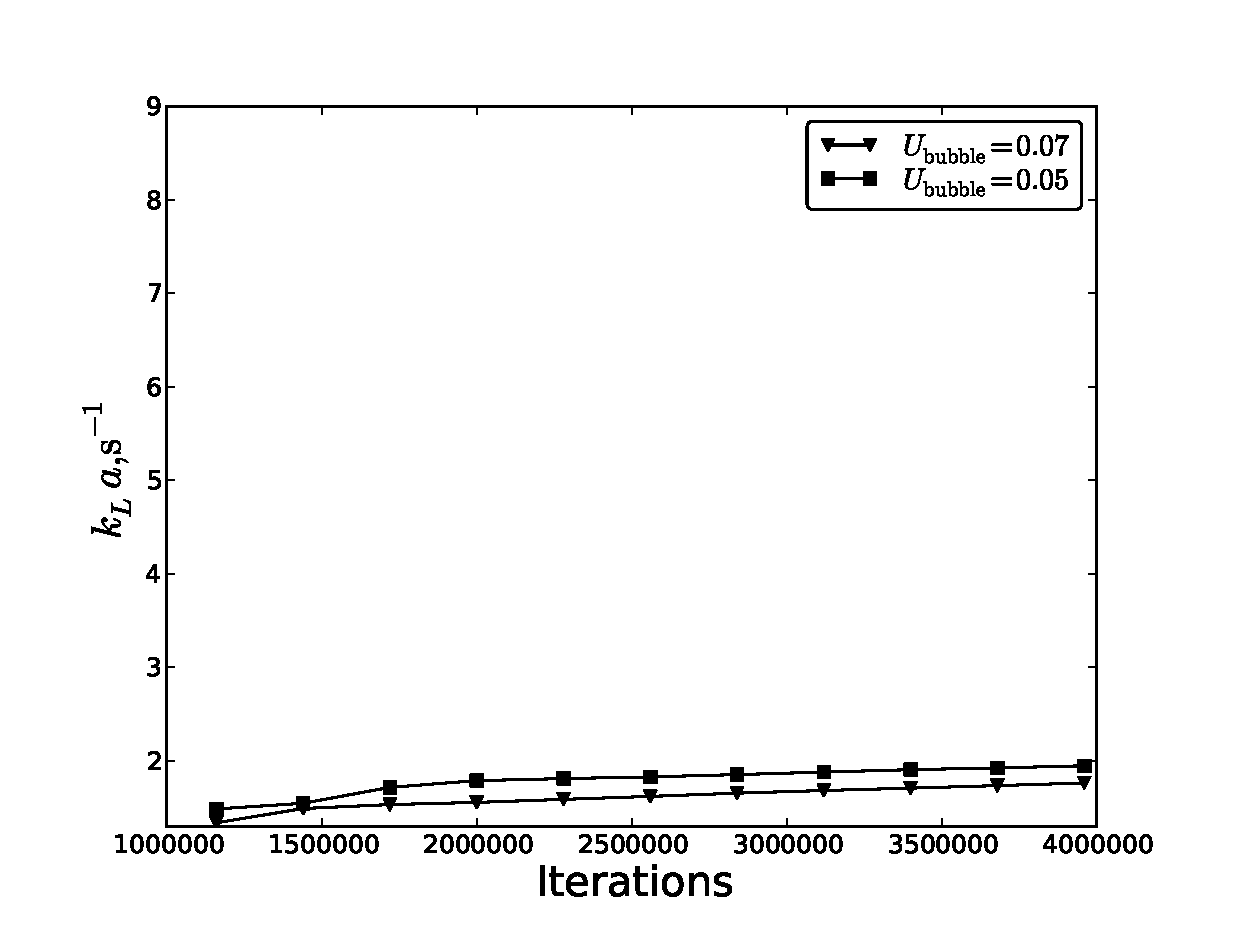
\includegraphics[width=0.5\textwidth]{Figures/steady_quadro_overall.eps}
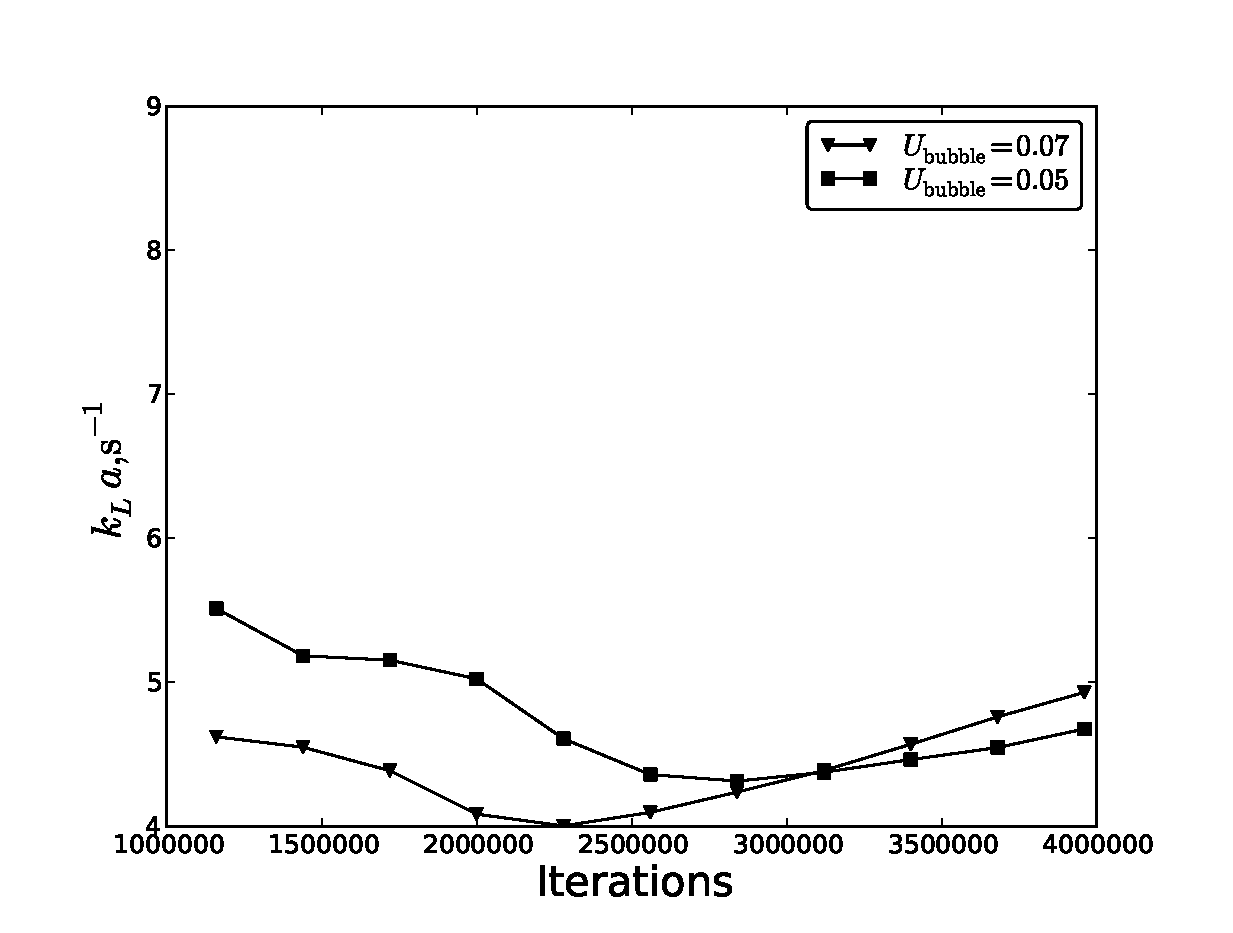
\includegraphics[width=0.5\textwidth]{Figures/steady_quadro_first.eps}\\
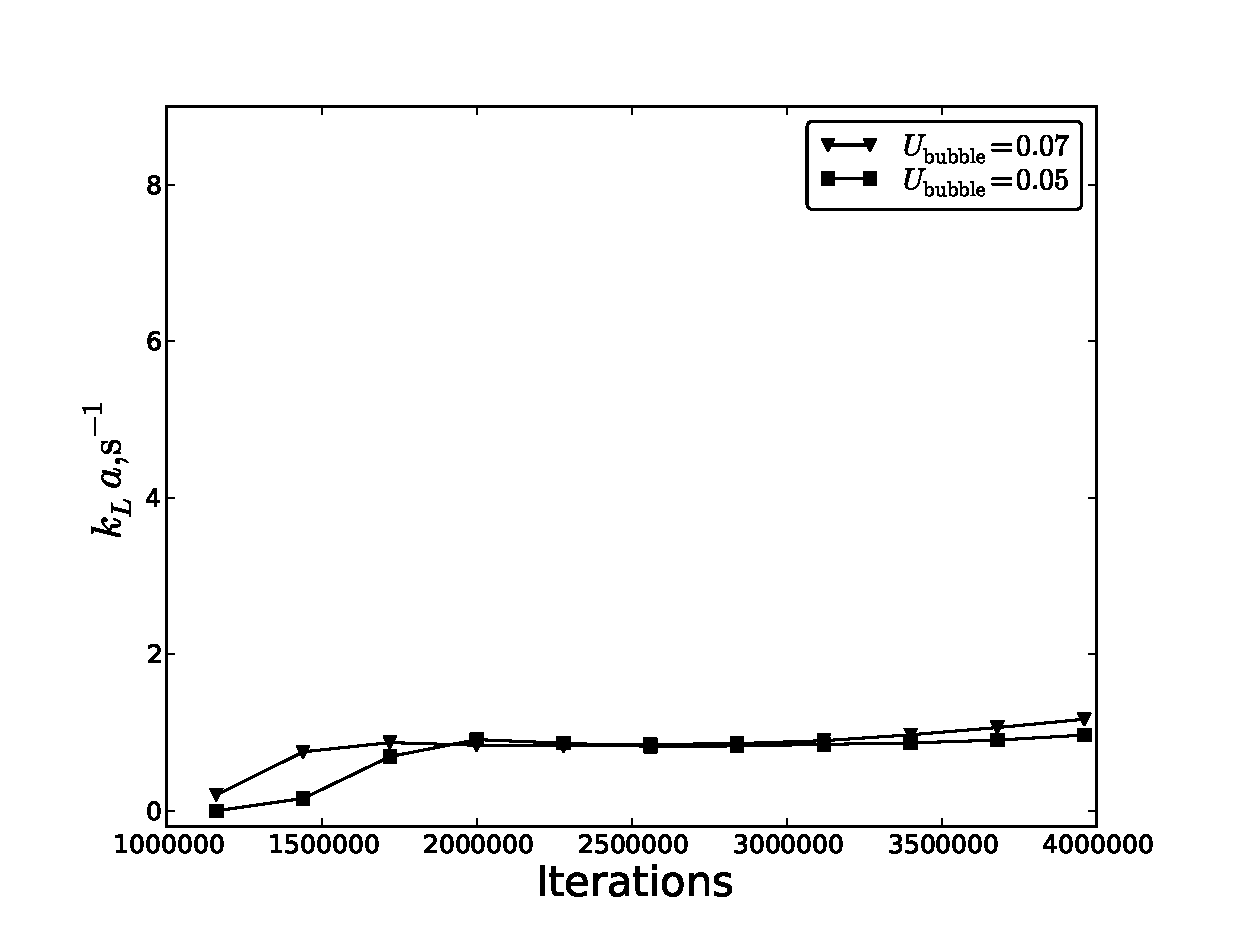
\includegraphics[width=0.5\textwidth]{Figures/steady_quadro_second.eps}
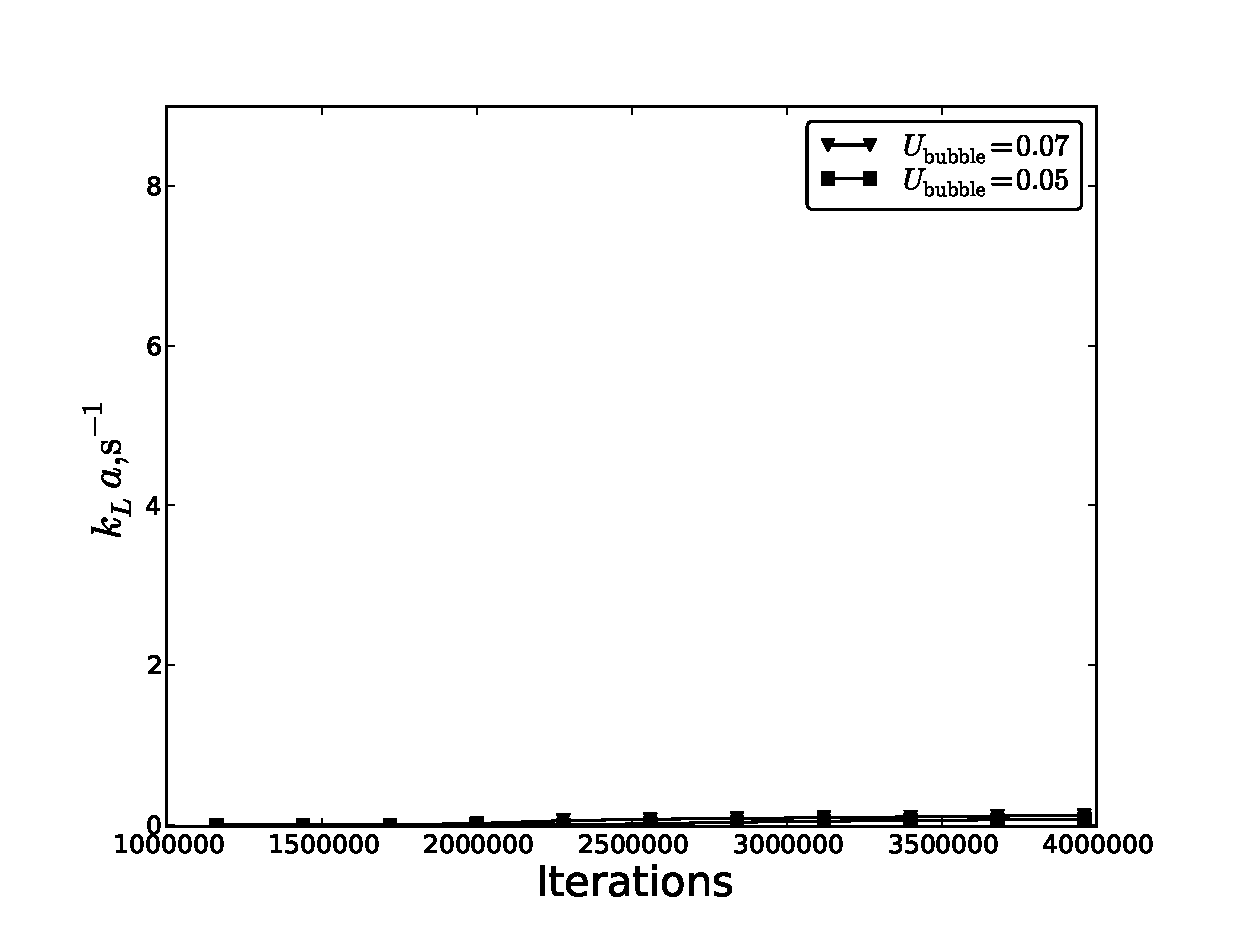
\includegraphics[width=0.5\textwidth]{Figures/steady_quadro_third.eps}\\
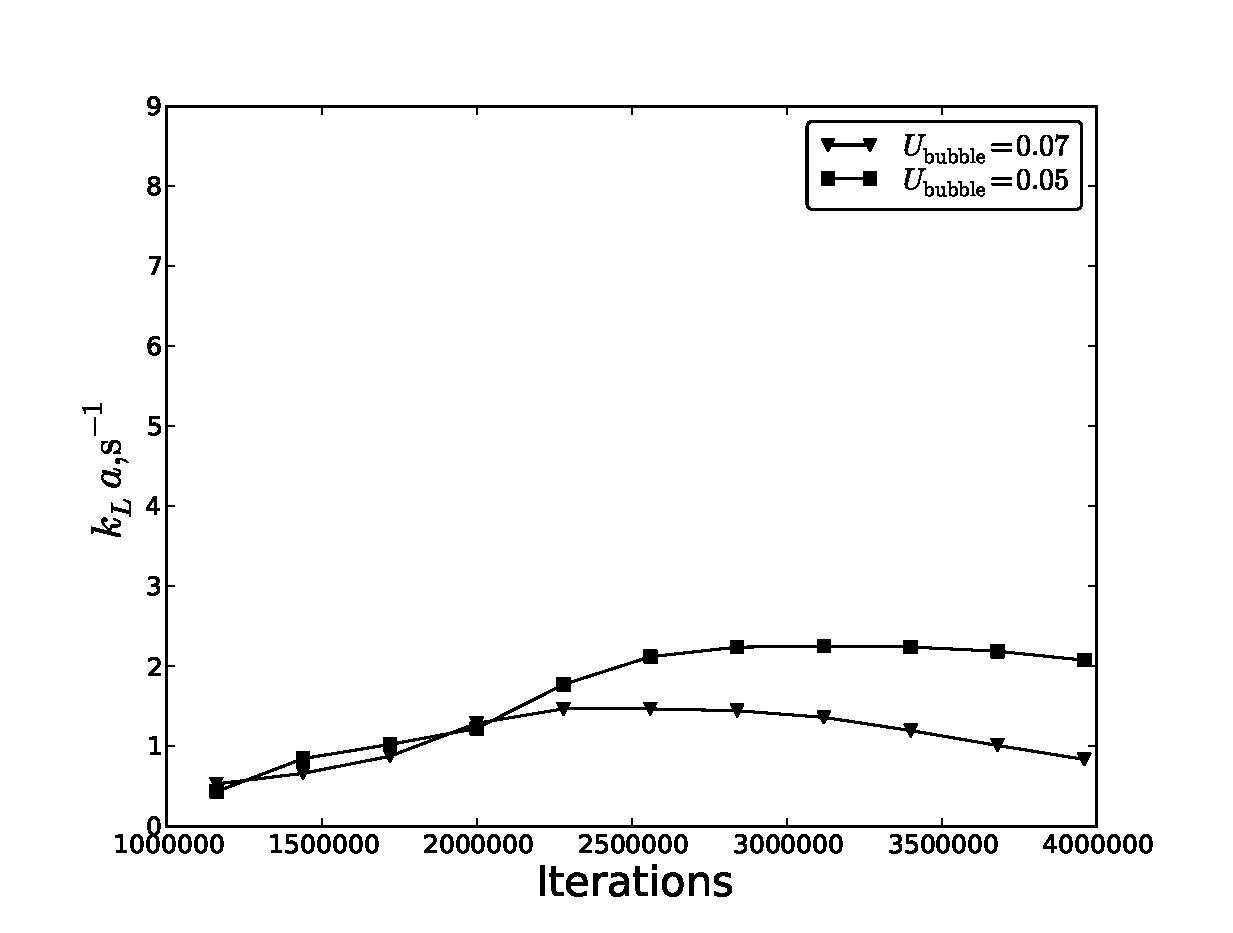
\includegraphics[width=0.5\textwidth]{Figures/steady_quadro_fourth.eps}\\
\caption{The mass transfer coefficient over time in different locations: overall mass transfer
coefficient (top left), first part (top right), second part (middle left), third part (middle
right) and fourth part (bottom left). \label{fig:results:quadro}}
\end{figure}

From Figs. \ref{fig:results:triple} and \ref{fig:results:quadro} one can see that $4,000,000$ time
steps are enough to saturate the second unit for $Ca=0.080$ number. Let us recall bubble velocities
and see what are the characteristic lengths for them calculated as time steps multiplied on the
bubble velocity. From the table one can see that each unit cell is saturated with the timesteps as
$1.5 \frac{N_x}{U_{bubble}}$ {\color{red}(Pretty important result)}. It's inevitably needs the
velocity increase.
\begin{table}[htb!]
\begin{tabularx}{\textwidth}{|X|X|X|X|X|X|X|X|}
\hline
$Ca$ &$U_{bubble}$ &$N_{iter_1}$ &$N_{iter_2}$ &$N_{iter_3}$ &$\frac{L_1}{N_x}$&$\frac{L_2}{N_x}$ 
&$\frac{L_3}{N_x}$\\
$0.026$&$0.0014$&$10^6$&$2\cdot10^6$&$4\cdot10^6$&$0.4666$ &$0.9333$ &$1.8666 $\\
$0.047$&$0.0027$&$10^6$&$2\cdot10^6$&$4\cdot10^6$&$0.9$    &$1.8$    &$3.6    $\\
$0.080$&$0.0045$&$10^6$&$2\cdot10^6$&$4\cdot10^6$&$1.5$    &$3.0$    &$6.0    $\\
$0.065$&$0.0037$&$10^6$&$2\cdot10^6$&$4\cdot10^6$&$1.2333$ &$2.4666$ &$4.9333 $\\
$0.222$&$0.0125$&$10^6$&$2\cdot10^6$&$4\cdot10^6$&$4.1666$ &$8.3333$ &$16.6666$\\
$0.479$&$0.0271$&$10^6$&$2\cdot10^6$&$4\cdot10^6$&$9.0333$ &$18.0666$&$36.1333$\\
$0.736$&$0.0416$&$10^6$&$2\cdot10^6$&$4\cdot10^6$&$13.8666$&$27.7333$&$55.4666$\\
$0.989$&$0.0559$&$10^6$&$2\cdot10^6$&$4\cdot10^6$&$18.6333$&$37.2666$&$74.5333$\\
\hline
\end{tabularx}
\caption{Table results to understand how many time steps are needed to be performed to reach the
saturation.\label{table:time:steps}}
\end{table}

\section{Lattice Boltzmann Benchmarks}
\citet{vanbaten-circular} represented a bubble with two hemisperes and a thin film. We want to
perform the benchmarking against these two representative cases.

\subsection{The radial case}
We want to examine the bounce-back conditions against the analytical solution. The system can be
prescribed by the following system of equations:
\beq
\begin{aligned}
&\partial_t C(r,t)=\frac{1}{r}\partial_r r \partial_r C(r,t)\\
&C(a,t)=C_0,\,C(r,0)=C_{init}
\end{aligned}
\feq 
The solution is represented as \cite{chemical-correlations}:
\beq
\frac{C(r,t)-C_{0}}{C_{init}-C_{0})}=\sum_{n=1}^{\infty}{\frac{2}{\mu_n
J_1(\mu_n)}\exp\Bigl(-\mu_n^2 \frac{D t}{a^2} \Bigr)J_0(\mu_n \frac{r}{a})},
\feq
where $\mu_n$ is the $n$-th zero root of the $0$th order Bessel polynomial $J_0(\mu_n)=0$. Some of
the corresponding roots are as follows: $\mu_1=2.4048$,$\mu_2=5.5201$,$\mu_3=8.6537$,
$\mu_4=11.7915$,$\mu_5=14.9309$.
By taking initial concentration to be $0$, one can obtain the following solution:
\beq
C(r,t)=C_0 \Biggl(1 - \sum_{n=1}^{\infty}{\frac{2}{\mu_n
J_1(\mu_n)}\exp\Bigl(-\mu_n^2 \frac{D t}{a^2} \Bigr)J_0(\mu_n \frac{r}{a})}\Biggr).
\feq

The solution depends only on the non-dimensional time: $\tau=\frac{D t}{a^2}$. Some examples for
different diffusion coefficients are presented in Fig.\ref{fig:cylinder:benchmark}.
\begin{figure}[htb!]
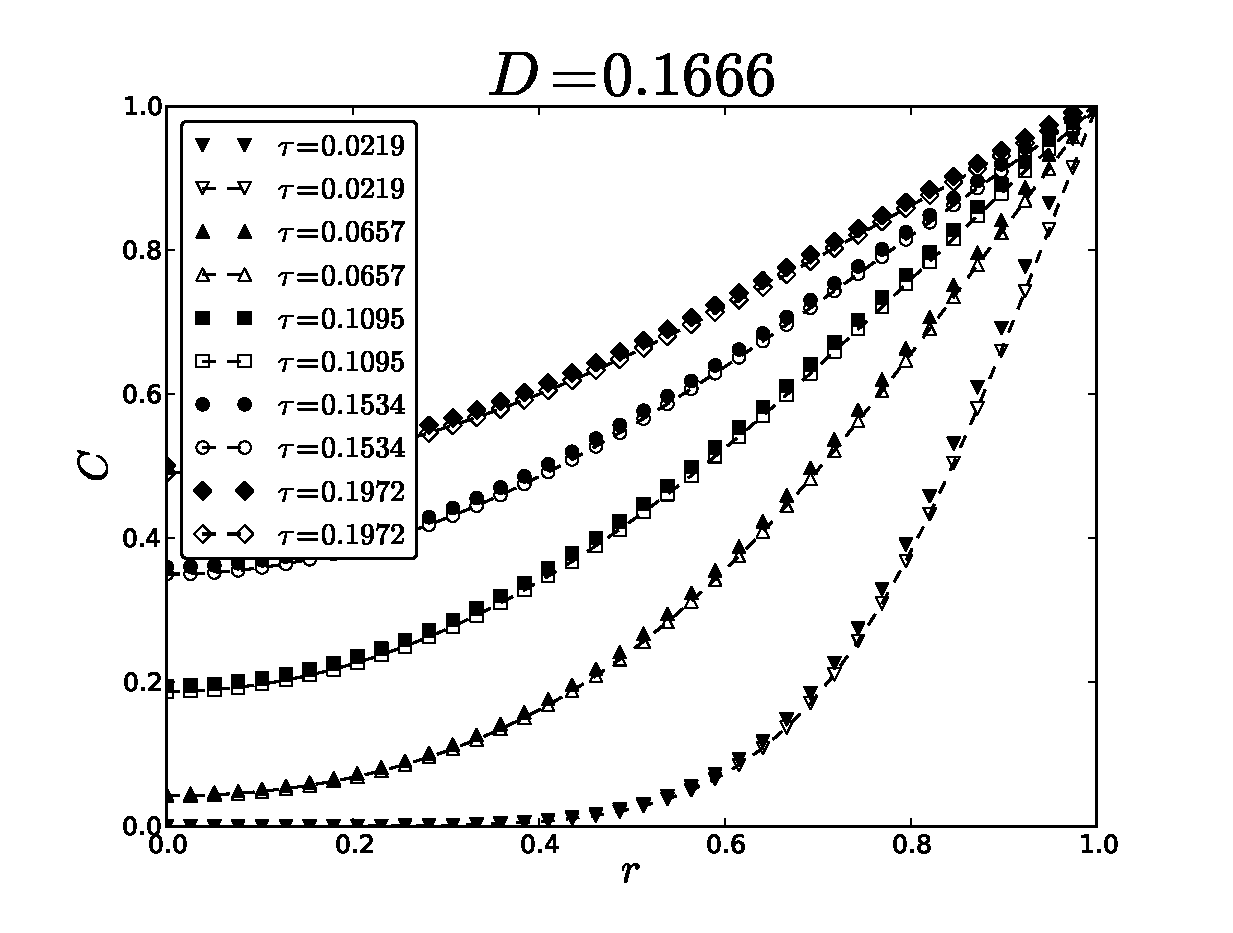
\includegraphics[width=0.5\textwidth]{Figures/cylinder1666.eps}
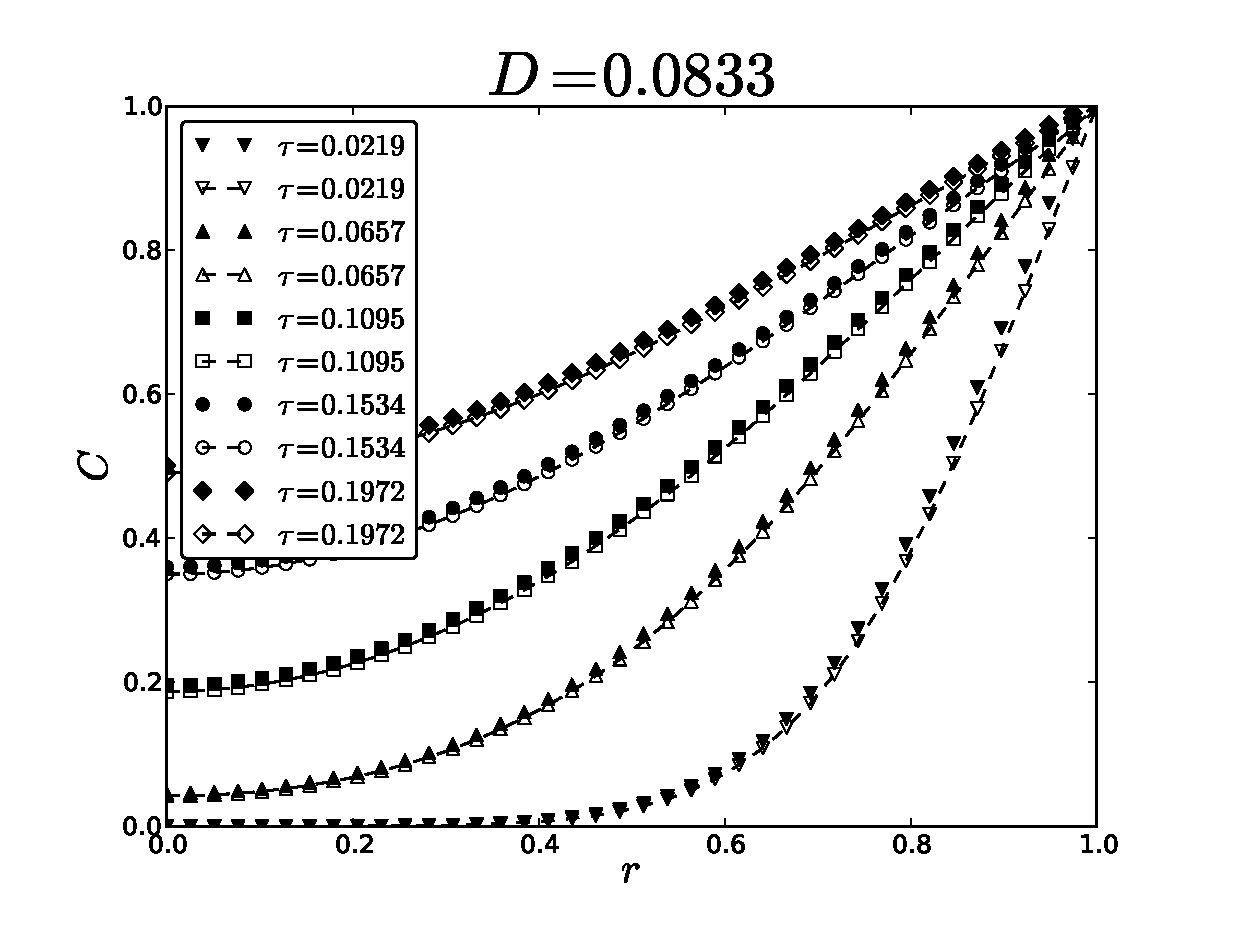
\includegraphics[width=0.5\textwidth]{Figures/cylinder0833.eps}\\
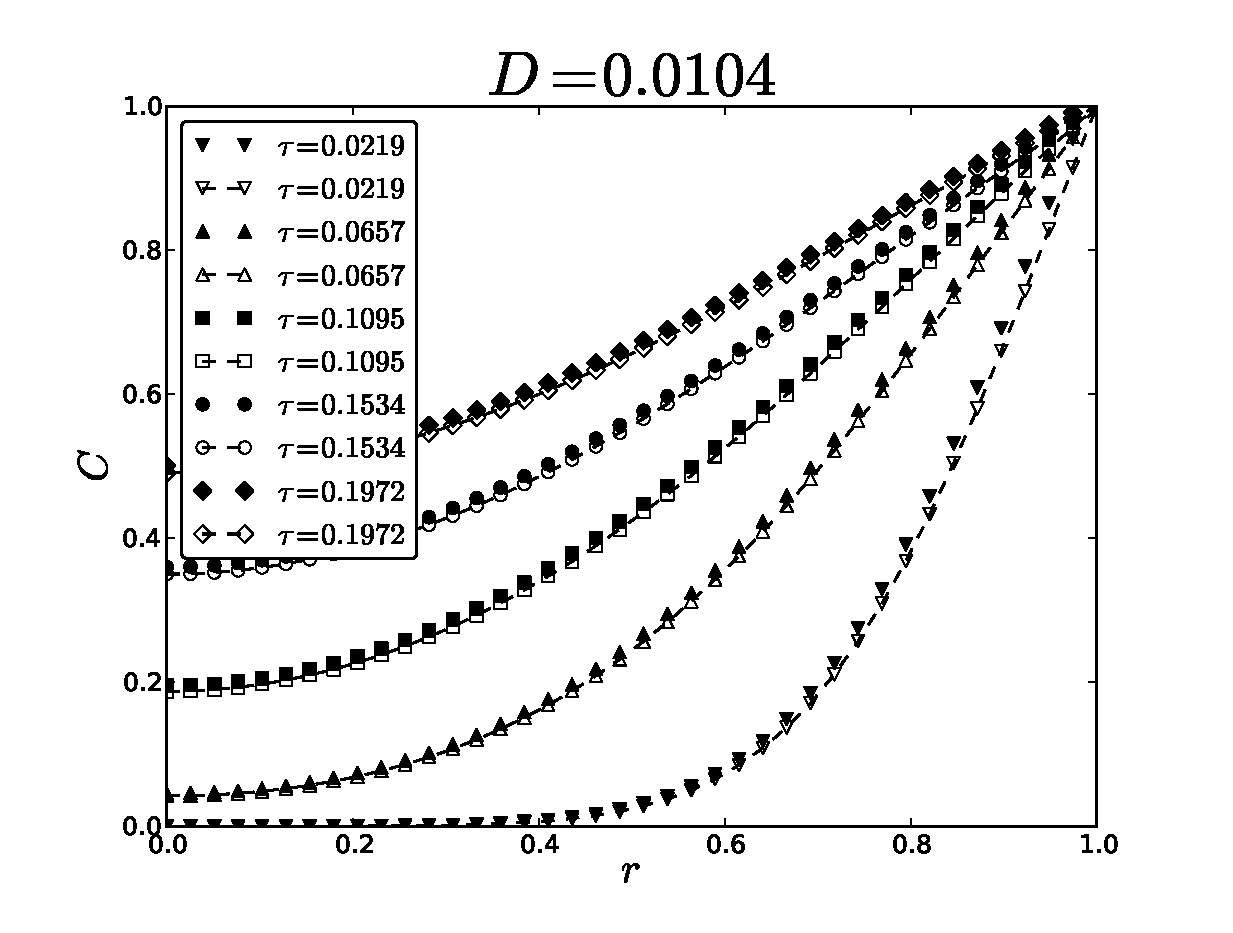
\includegraphics[width=0.5\textwidth]{Figures/cylinder0104.eps}
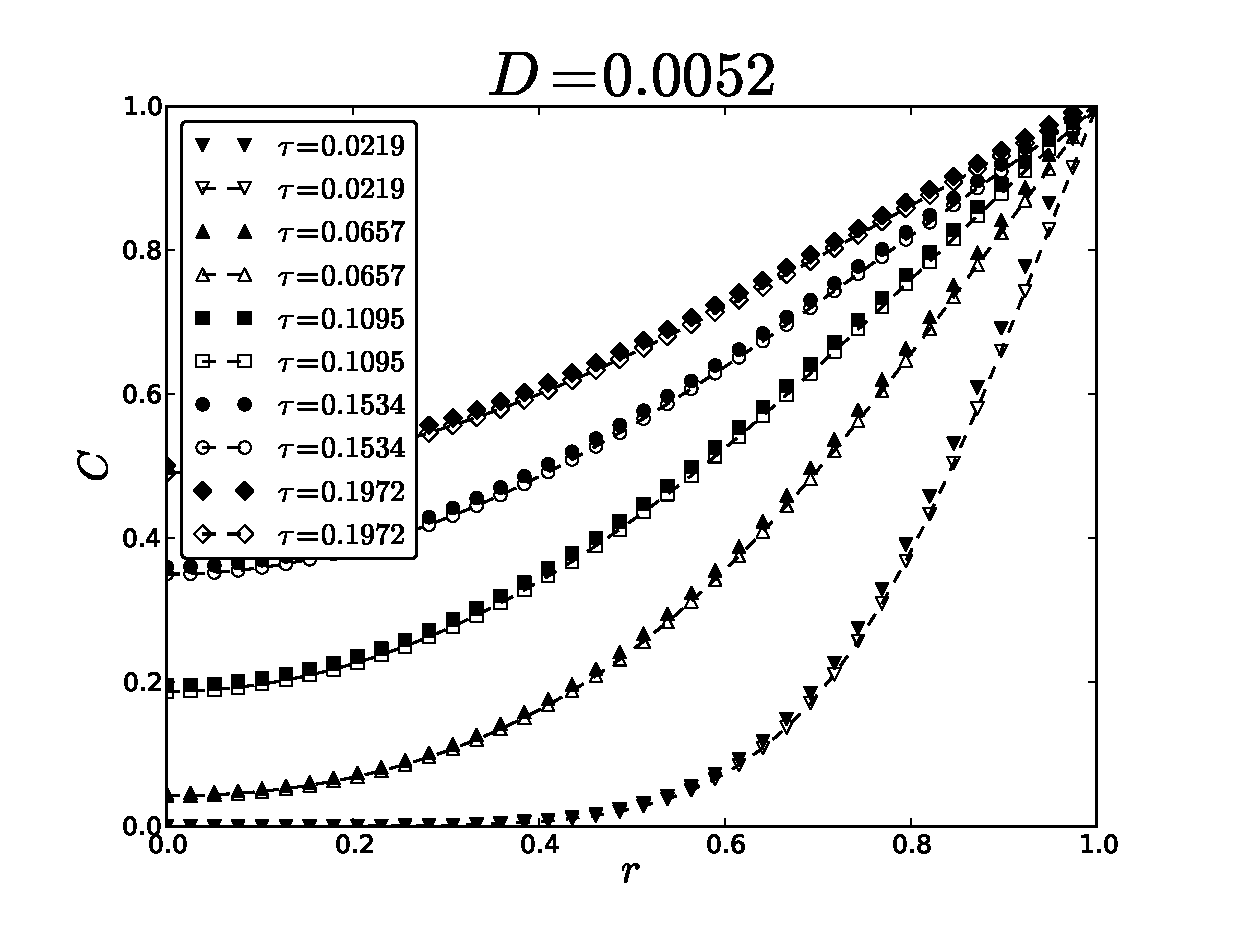
\includegraphics[width=0.5\textwidth]{Figures/cylinder0052.eps}\\
\caption{Profiles for different diffusion parameters. One can see that the diffusion is captured
accurately in non-dimensional space \label{fig:cylinder:benchmark}.}
\end{figure}



\section{Tweaking velocity}
This section does the job of increasing velocity results. The ulimate goal is to increase velocity
to about $20-50$ times for velocity while keeping dimensionless parameters the same. The
nondimensional parameter Peclet number governs the advection-diffusion equation:
\beq
Pe=\frac{U_{bubble} N_y}{D},
\feq
where $D$ is the diffusion coefficient to prescribe. As far as we want to increase velocity, that
means one needs to increase the diffusion coefficient as well. We make a few runs with velocities
$5,10,20,40$ times larger than original velocities. 


\bibliographystyle{unsrtnat}
\bibliography{paper}

\end{document}

